% !TeX root = ../main.tex
% Add the above to each chapter to make compiling the PDF easier in some editors.

\chapter{Online Algorithms}\label{chapter:online_algorithms}

In this chapter, we discuss the online algorithms we implemented in our work. Similar to the previous chapter on offline algorithms, we begin our discussion in \cref{section:online_algorithms:ud} with algorithms for the uni-dimensional setting. As was discussed in \cref{chapter:theory}, these algorithms give strong guarantees yielding a constant competitive ratio. Next in \cref{section:online_algorithms:md}, we extend our discussion to the multi-dimensional setting. Here, the guarantees are not as strong. We thus begin in \cref{section:online_algorithms:md:lazy_budgeting} by considering lazy budgeting algorithms for smoothed convex optimization problems with particular cost functions. As mentioned previously in \cref{chapter:theory}, while there are algorithms with sublinear regret (gradient descent), there cannot be any algorithms achieving a dimension-independent constant competitive ratio unless the class of allowed cost functions is restricted~\cite{Chen2018}. In \cref{section:online_algorithms:md:descent_methods}, we thus discuss gradient methods that perform well with regard to either the competitive ratio or regret with a restricted class of cost functions. Still, sublinear regret and a constant competitive ratio cannot be achieved simultaneously, even for linear cost functions~\cite{Andrew2015}. We, therefore, end this chapter in \cref{section:online_algorithms:md:predictions} with a discussion of algorithms that use predictions to circumvent this fundamental limitation. \Cref{appendix:taxonomy} includes an overview of all discussed online algorithms.

Throughout this chapter, we denote by $\tau \in [T]$ the current time slot. In contrast to offline algorithms that know the hitting costs $f_t$ for all $t \in [T]$, an online algorithm only knows the hitting costs $f_t$ up to $\tau$, i.e. $t \in [\tau]$.

\section{Uni-Dimensional}\label{section:online_algorithms:ud}

\subsection{Lazy Capacity Provisioning}\label{section:online_algorithms:ud:lazy_capacity_provisioning}

\subsubsection{Fractional Algorithm}

We begin by returning to the notion of capacity provisioning that we introduced in \cref{section:offline_algorithms:ud:capacity_provisioning}, yielding a backward-recurrent algorithm finding an optimal schedule for SSCO. This algorithm computed bounds $X_{\tau}^L$ and $X_{\tau}^U$ on the optimal solution, which only depend on the schedule up to time slot $\tau$. However, the optimal offline algorithm stayed within these bounds moving backward in time which is impossible for an online algorithm. \citeauthor*{Lin2011}~\cite{Lin2011} present a similar algorithm moving forward in time called \emph{lazy capacity provisioning}. We compute the schedule $X_{\tau}$ during time slot $\tau$ by setting $X_{\tau} = X_{\tau-1}$ unless this violates the bounds in which case we make the smallest possible change: \begin{align*}
    X_{\tau} = \begin{cases} 
        0 & \tau \leq 0 \\
        (X_{\tau-1})_{X_{\tau,\tau}^L}^{X_{\tau,\tau}^U} & \tau \geq 1
    \end{cases}
\end{align*} where $(X_{\tau-1})_{X_{\tau,\tau}^L}^{X_{\tau,\tau}^U}$ is the projection of $X_{\tau-1}$ onto $[X_{\tau,\tau}^L, X_{\tau,\tau}^U]$~\cite{Lin2011}. \Cref{fig:backward_recurrent_capacity_provisioing_vs_lazy_capacity_provisioning} shows how this update rule differs from \nameref{alg:brcp}. The resulting algorithm is described in \cref{alg:ud:lcp}. Similar to the offline algorithm, we can use algorithms for convex optimization to compute the upper and lower bounds. Hence, we obtain a complexity of $\mathcal{O}(\tau C O_{\epsilon}^{\tau})$ for $\epsilon$-optimal upper and lower bounds. This complexity is worrying as it depends on $\tau$, which may grow very large. However, \citeauthor*{Lin2011}~\cite{Lin2011} prove the following lemma, which implies that it suffices to compute the lower and upper bounds using only the history since the last time slot where both bounds were either decreased or increased.

\begin{figure}
    \centering
    % This file was created by tikzplotlib v0.9.9.
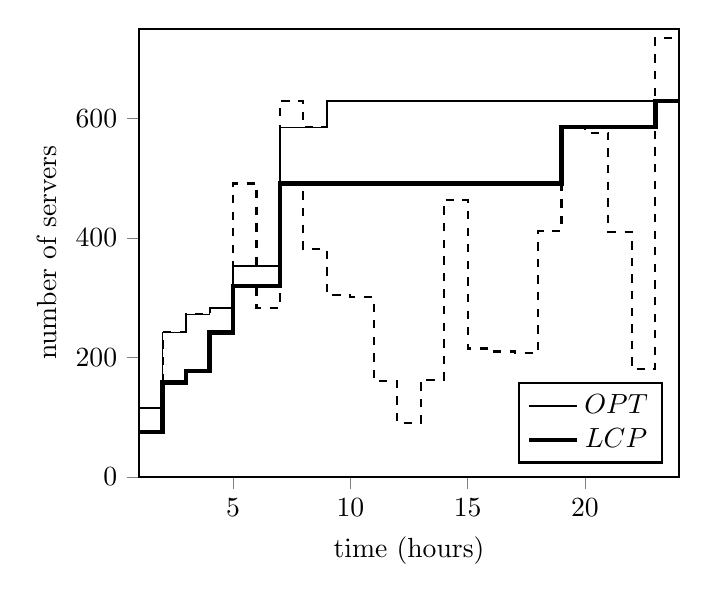
\begin{tikzpicture}

\begin{axis}[
legend pos=south east,
tick align=outside,
tick pos=left,
% x grid style={white!69.0196078431373!black},
xlabel={time (hours)},
xmin=1, xmax=24,
% xtick style={color=black},
% y grid style={white!69.0196078431373!black},
ylabel={number of servers},
ymin=0, ymax=750,
% ytick style={color=black}
]
\addplot [semithick, black, const plot mark left]
table {%
1 115
2 242
3 272
4 283
5 353
6 353
7 585
8 585
9 629
10 629
11 629
12 629
13 629
14 629
15 629
16 629
17 629
18 629
19 629
20 629
21 629
22 629
23 629
24 629
};
\addlegendentry{$OPT$}
\addplot [ultra thick, black, const plot mark left]
table {%
1 75
2 158
3 177
4 242
5 320
6 320
7 491
8 491
9 491
10 491
11 491
12 491
13 491
14 491
15 491
16 491
17 491
18 491
19 586
20 586
21 586
22 586
23 629
24 629
};
\addlegendentry{$LCP$}
\addplot [dashed, black, const plot mark left]
table {%
1 75
2 158
3 177
4 242
5 320
6 283
7 491
8 381
9 304
10 301
11 160
12 90
13 163
14 464
15 215
16 210
17 207
18 411
19 586
20 576
21 410
22 180
23 629
24 629
};
\addplot [dashed, black, const plot mark left]
table {%
1 115
2 242
3 272
4 283
5 491
6 353
7 629
8 585
9 629
10 629
11 629
12 629
13 629
14 629
15 629
16 629
17 629
18 629
19 629
20 629
21 629
22 629
23 734
24 734
};
\end{axis}

\end{tikzpicture}

    \caption{Backward-Recurrent Capacity Provisioning vs. Lazy Capacity Provisioning. LCP stays within the bounds ``lazily'' moving forwards in time. The optimal solution stays within the bounds moving backwards in time.}
    \label{fig:backward_recurrent_capacity_provisioing_vs_lazy_capacity_provisioning}
\end{figure}

\begin{lemma}
\cite{Lin2011} If there exists an index $t \in [1, \tau-1]$ such that $X_{\tau,t+1}^U < X_{\tau,t}^U$ or $X_{\tau,t+1}^L > X_{\tau,t}^L$, then $(\hat{X}_{\tau,1},\dots,\hat{X}_{\tau,t}) := (X_{\tau,1}^L,\dots,X_{\tau,t}^L) = (X_{\tau,1}^U,\dots,X_{\tau,t}^U)$, and no matter what the future arrival is, solving the optimization in $[1,\tau']$ for $\tau' > \tau$ is equivalent to solving two optimizations: one over $[1,t]$ with initial condition $X_0$ and final condition $\hat{X}_{\tau,t}$ and the second over $[t+1,\tau']$ with initial condition $\hat{X}_{\tau,t}$.
\end{lemma}

While not changing the worst-case complexity, this significantly improves the practical complexity in the application of right-sizing data centers as diurnal load patterns typically ensure that less than a day needs to be considered~\cite{Lin2011}. We denote by $X_{\tau}^{L,(t,x_0)}$ and $X_{\tau}^{U,(t,x_0)}$ the bounds resulting from optimizations beginning at time slot $t$ with initial condition $x_0$. \citeauthor*{Lin2011}~\cite{Lin2011} showed that lazy capacity provisioning is $3$-competitive and also proved that this result is tight.

\begin{algorithm}
    \caption{Lazy Capacity Provisioning~\cite{Lin2011}}\label{alg:ud:lcp}
    \SetKwInOut{Input}{Input}
    \Input{$\mathcal{I}_{\text{SSCO}} = (\tau \in \mathbb{N}, m \in \mathbb{N}, \beta \in \mathbb{R}_{>0}, (f_1, \dots, f_{\tau}) \in (\mathbb{R}_{\geq 0} \to \mathbb{R}_{\geq 0})^{\tau})$}
    $t_0 \gets 0$\;
    $x_0 \gets 0$\;
    \For{$t \gets \tau-1$ \KwTo $2$}{
        \If{$X_{t,t}^U < X_{t,t-1}^U \lor X_{t,t}^L > X_{t,t-1}^L$}{
            $t_0 \gets t$\;
            $x_0 \gets X_{t,t-1}^U$\;
            \KwBreak
        }
    }
    find $X_{\tau,\tau}^{L,(t_0,x_0)}$ using the optimization described by \cref{eq:ud:brcp:lower}\;
    find $X_{\tau,\tau}^{U,(t_0,x_0)}$ using the optimization described by \cref{eq:ud:brcp:upper}\;
    \Return $(X_{\tau-1})_{X_{\tau,\tau}^{L,(t_0,x_0)}}^{X_{\tau,\tau}^{U,(t_0,x_0)}}$\;
\end{algorithm}

\subsubsection{Integral Algorithm}

\citeauthor*{Albers2018}~\cite{Albers2018} applied lazy capacity provisioning to the integral variant Int-SSCO using their graph-based offline algorithm discussed in \cref{section:offline_algorithms:ud:graph_based} to compute the integral lower and upper bounds. It is apparent that this immediately yields a deterministic online algorithm for Int-SSCO. \citeauthor*{Albers2018}~\cite{Albers2018} showed that similar to lazy capacity provisioning, their algorithm is $3$-competitive. Due to the changed method of determining the bounds, its runtime is $\mathcal{O}(\tau^2 C \log_2 m)$. Note that it is impossible to cache the intermediate results of the dynamic program (see \cref{alg:ud:optimal_graph_search}) as the binary search over possible configurations considers different vertices depending on the obtained schedule, which changes over time. Thus, for large $\tau$, it may be beneficial to use caching instead of binary search resulting in a worst-case runtime of $\mathcal{O}(\tau C m)$. By using the same method of shortening the used history that was proposed by \citeauthor*{Lin2011}~\cite{Lin2011}, we can reduce this time complexity drastically in practice (for large $\tau$). Thus, the adopted algorithm is still described by \cref{alg:ud:lcp}. We simply need to slightly modify the graph-based algorithm computing optimal offline solutions to allow for initial conditions other than $0$.

\subsection{Memoryless Algorithm}\label{section:online_algorithms:ud:memoryless}

\citeauthor*{Bansal2015}~\cite{Bansal2015} showed that for SSCO, a competitive ratio of $3$ can also be attained by a memoryless algorithm. In a memoryless online algorithm for smoothed convex optimization, the configuration $X_{\tau}$ only depends on the preceding configuration $X_{\tau-1}$ and the current hitting cost $f_{\tau}$. This generally allows for a more space and time-efficient algorithm, which is important when choosing a small time slot length $\delta$ to be more responsive to changes in load.

The algorithm proposed by \citeauthor*{Bansal2015}~\cite{Bansal2015} works as follows. Let $\hat{x}$ be the minimizer of $f_{\tau}(x)$, i.e. $\hat{x} = \argmin_{x \in \mathcal{X}} f_{\tau}(x)$. The algorithm moves into the direction of the minimizer until it either reaches $\hat{x}$, or it reaches a configuration $x$ where its switching cost equals twice the hitting cost of $x$. \Cref{fig:memoryless_algorithm} gives an example of a step of the algorithm. We observe that this is equivalent to the following convex optimization: \begin{align}\label{eq:ud:memoryless}\begin{aligned}
    &\min_{x \in \mathcal{X}} &&f_{\tau}(x) \\
    &\text{subject to}        &&\beta |x - X_{\tau-1}| \leq \frac{f_{\tau}(x)}{2}.
\end{aligned}\end{align} Originally, \citeauthor*{Bansal2015}~\cite{Bansal2015} proposed this algorithm for a restricted variant of uni-dimensional SSCO where the decision space is unbounded, i.e., $\mathcal{X} = \mathbb{R}$, and the switching costs are given by the $\ell_1$ norm. In particular, they choose $\beta = 1$. First, it is easy to see that we can adapt the algorithm for a bounded decision space by bounding the feasible region of the optimization problem in \cref{eq:ud:memoryless}. Second, we observe that $\beta$ can simply be interpreted as the weight that we associate with smoothing (i.e., minimizing movement) instead of minimizing hitting costs. This is shown by the following equation, which is obtained by dividing the cost of \cref{eq:simplified_smoothed_convex_optimization} by $\beta$: \begin{align}\label{eq:simplified_smoothed_convex_optimization:without_beta}
    \sum_{t=1}^T \frac{1}{\beta} f_t(X_t) + \sum_{k=1}^d (X_{t,k} - X_{t-1,k})^+.
\end{align} The cost associated with this equation is the cost of \cref{eq:simplified_smoothed_convex_optimization} linearly scaled by $1 / \beta$. Especially, this argument shows the following lemma.

\begin{lemma}\label{lemma:switching_cost_absolute_vs_positive_movement}
A schedule is optimal with respect to \cref{eq:simplified_smoothed_convex_optimization:without_beta} if and only if it is optimal with respect to \cref{eq:simplified_smoothed_convex_optimization}.
\end{lemma}

Therefore, without loss of optimality, we can incorporate the weight of the switching cost beta into the hitting costs. Further, note that in their model, \citeauthor*{Bansal2015}~\cite{Bansal2015} consider the absolute movement, i.e. $|X_{t,k} - X_{t-1,k}|$, rather than only positive movements, i.e. $(X_{t,k} - X_{t-1,k})^+$. However, with \cref{lemma:switching_cost_l1_norm_vs_pos_movement} in \cref{chapter:theory}, we have shown that these switching costs only differ by a constant factor (namely $1/2$).

The resulting algorithm is simply given by determining $\hat{x}$ based on the convex optimization in \cref{eq:ud:memoryless}, see \cref{alg:ud:memoryless}. Thus, the time (and space) complexity of this memoryless algorithm is $\mathcal{O}(C O_{\epsilon}^1)$ for finding $\epsilon$-optimal solutions.

\begin{figure}
    \centering
    


\tikzset{every picture/.style={line width=0.75pt}} %set default line width to 0.75pt

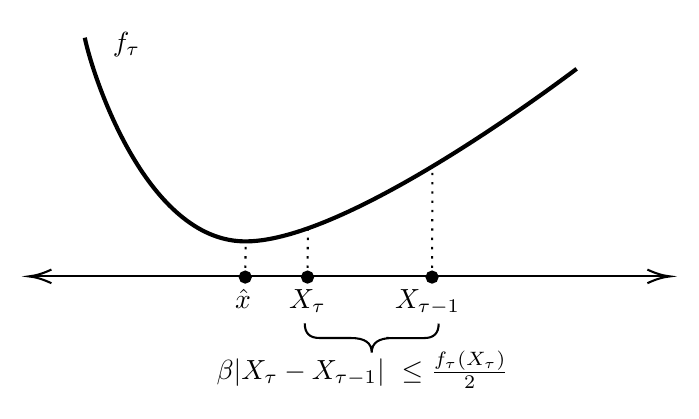
\begin{tikzpicture}[x=0.75pt,y=0.75pt,yscale=-1,xscale=1]
%uncomment if require: \path (0,308); %set diagram left start at 0, and has height of 308

%Curve Lines [id:da37061921880533877]
\draw [line width=1.5]    (98,85.33) .. controls (102.36,105.81) and (127.25,179.72) .. (172,183.33) .. controls (216.75,186.95) and (312.43,117.26) .. (335,100.33) ;
%Straight Lines [id:da8132100594867722]
\draw    (73,200.33) -- (378,200.33) ;
\draw [shift={(380,200.33)}, rotate = 180] [color={rgb, 255:red, 0; green, 0; blue, 0 }  ][line width=0.75]    (10.93,-3.29) .. controls (6.95,-1.4) and (3.31,-0.3) .. (0,0) .. controls (3.31,0.3) and (6.95,1.4) .. (10.93,3.29)   ;
\draw [shift={(71,200.33)}, rotate = 0] [color={rgb, 255:red, 0; green, 0; blue, 0 }  ][line width=0.75]    (10.93,-3.29) .. controls (6.95,-1.4) and (3.31,-0.3) .. (0,0) .. controls (3.31,0.3) and (6.95,1.4) .. (10.93,3.29)   ;
%Shape: Circle [id:dp2801837798690885]
\draw  [fill={rgb, 255:red, 0; green, 0; blue, 0 }  ,fill opacity=1 ] (172.67,200.67) .. controls (172.67,199.19) and (173.86,198) .. (175.33,198) .. controls (176.81,198) and (178,199.19) .. (178,200.67) .. controls (178,202.14) and (176.81,203.33) .. (175.33,203.33) .. controls (173.86,203.33) and (172.67,202.14) .. (172.67,200.67) -- cycle ;
%Shape: Circle [id:dp9237316574850754]
\draw  [fill={rgb, 255:red, 0; green, 0; blue, 0 }  ,fill opacity=1 ] (262.67,200.67) .. controls (262.67,199.19) and (263.86,198) .. (265.33,198) .. controls (266.81,198) and (268,199.19) .. (268,200.67) .. controls (268,202.14) and (266.81,203.33) .. (265.33,203.33) .. controls (263.86,203.33) and (262.67,202.14) .. (262.67,200.67) -- cycle ;
%Shape: Circle [id:dp045787056716331875]
\draw  [fill={rgb, 255:red, 0; green, 0; blue, 0 }  ,fill opacity=1 ] (202.67,200.67) .. controls (202.67,199.19) and (203.86,198) .. (205.33,198) .. controls (206.81,198) and (208,199.19) .. (208,200.67) .. controls (208,202.14) and (206.81,203.33) .. (205.33,203.33) .. controls (203.86,203.33) and (202.67,202.14) .. (202.67,200.67) -- cycle ;
%Straight Lines [id:da9850850655894281]
\draw    [dash pattern={on 0.84pt off 2.51pt}]  (175.33,200.67) -- (175.52,184.05) ;
%Straight Lines [id:da4019047700825191]
\draw    [dash pattern={on 0.84pt off 2.51pt}]  (205.33,200.67) -- (205.52,177.05) ;
%Straight Lines [id:da23167830177054616]
\draw    [dash pattern={on 0.84pt off 2.51pt}]  (265.33,200.67) -- (265.52,147.05) ;
%Shape: Brace [id:dp024365056849508404]
\draw   (204,223) .. controls (204,227.67) and (206.33,230) .. (211,230) -- (226.26,230.02) .. controls (232.93,230.02) and (236.26,232.35) .. (236.25,237.02) .. controls (236.26,232.35) and (239.59,230.02) .. (246.26,230.03)(243.26,230.03) -- (261.52,230.04) .. controls (266.19,230.05) and (268.52,227.72) .. (268.52,223.05) ;

% Text Node
\draw (169,205) node [anchor=north west][inner sep=0.75pt]    {$\hat{x}$};
% Text Node
\draw (195,205) node [anchor=north west][inner sep=0.75pt]    {$X_{\tau }$};
% Text Node
\draw (246,205) node [anchor=north west][inner sep=0.75pt]    {$X_{\tau -1}$};
% Text Node
\draw (160,235) node [anchor=north west][inner sep=0.75pt]    {$\beta |X_{\tau } -X_{\tau -1} |\ \leq \frac{f_{\tau }( X_{\tau })}{2}$};
% Text Node
\draw (110,81) node [anchor=north west][inner sep=0.75pt]    {$f_{\tau }$};


\end{tikzpicture}

    \caption{The memoryless algorithm moves towards the minimizer of the hitting cost, balancing hitting and movement costs.}
    \label{fig:memoryless_algorithm}
\end{figure}

\begin{algorithm}
    \caption{Memoryless algorithm~\cite{Bansal2015}}\label{alg:ud:memoryless}
    \SetKwInOut{Input}{Input}
    \Input{$\mathcal{I}_{\text{SSCO}} = (\tau \in \mathbb{N}, m \in \mathbb{N}, \beta \in \mathbb{R}_{>0}, (f_1, \dots, f_{\tau}) \in (\mathbb{R}_{\geq 0} \to \mathbb{R}_{\geq 0})^{\tau})$}
    \Return $\hat{x}$ such that that $\hat{x}$ is the result of the optimization in \cref{eq:ud:memoryless}\;
\end{algorithm}

\subsection{Probabilistic Algorithm}\label{section:online_algorithms:ud:probabilistic}

Next, we discuss a $2$-competitive algorithm developed by \citeauthor*{Bansal2015}~\cite{Bansal2015}, which works by maintaining a probability distribution over configurations. Using this probability distribution, they describe a randomized algorithm which they subsequently translate into a deterministic algorithm. We discuss how to gather a randomized and then a deterministic algorithm from a probability distribution. Then, we describe how \citeauthor*{Bansal2015}~\cite{Bansal2015} determine the probability distribution and how it can be computed in practice.

\subsubsection{From Probability Distribution to Deterministic Algorithm}

Let's suppose we have given a probability distribution $p$ over configurations $x \in \mathcal{X}$. A randomized algorithm is then described by initially picking a number $\gamma \in [0,1]$ uniformly at random and then maintaining the invariant that at time $\tau$ the chosen configuration $x_{\tau}$ has the property that the probability mass to the left of $x_{\tau}$ with respect to $p$ is exactly $\gamma$~\cite{Bansal2015}. Crucially, this approach only works in the fractional setting. Also, note that $\gamma$ is chosen only once prior to running the algorithm. This describes how we obtain a randomized algorithm from a probability distribution over configurations.

Next, \citeauthor*{Bansal2015}~\cite{Bansal2015} show the following theorem, which describes how we can obtain a deterministic algorithm from a randomized algorithm. \begin{theorem}
   ~\cite{Bansal2015} For the problem of (fractional) online convex optimization, if there exists a $\rho$-competitive randomized algorithm $\mathcal{R}$ then there exists a $\rho$-competitive deterministic algorithm $\mathcal{D}$.
\end{theorem}
\begin{proof}
\citeauthor*{Bansal2015}~\cite{Bansal2015} prove this theorem using Jensen's inequality. In the setting of a probability space, \emph{Jensen's inequality}\index{Jensen's inequality} claims that given a convex function $\varphi$ and a random variable $X$ we have \begin{align}
    E(\varphi(X)) \geq \varphi(E X)
\end{align} provided both expectations exist, i.e. $E |X|$ and $E |\varphi(X)| < \infty$~\cite{Durrett2010}.

Let $X_{\tau}$ be a random variable denoting the configuration of the randomized algorithm $\mathcal{R}$ at time $\tau$. Then, the deterministic algorithm $\mathcal{D}$ of \citeauthor*{Bansal2015}~\cite{Bansal2015} sets their configuration to $x_{\tau} = E X_{\tau}$. The cost of $\mathcal{D}$ is thus given by $f_{\tau}(x_{\tau}) + (x_{\tau} - x_{\tau-1})^+$ and the cost of $\mathcal{R}$ is given by $E(f_{\tau}(X_{\tau})) + E((X_{\tau} - X_{\tau-1})^+)$. We observe that both $f_{\tau}$ and $(\cdot)^+$ are convex functions, implying that the cost of $\mathcal{R}$ is at least $f_{\tau}(E X_{\tau}) + (E X_{\tau} - E X_{\tau-1})^+$ which equals the cost of $\mathcal{D}$. Summing over all $t$ completes the proof.
\end{proof}

Hence, we have seen that a deterministic algorithm can be obtained from a randomized algorithm by, in each time slot, choosing the expected configuration of the randomized algorithm.

\subsubsection{Assumptions}

In the description of their algorithm, \citeauthor*{Bansal2015}~\cite{Bansal2015} consider a restricted variant of uni-dimensional SSCO. Similar to their memoryless algorithm, which we discussed in \cref{section:online_algorithms:ud:memoryless}, they consider an unbounded decision space, i.e., $\mathcal{X} = \mathbb{R}$, and the $\ell_1$ norm as switching costs. Further, for their description of this probabilistic algorithm, they assume that the minimizer $\hat{x}$ of $f_{\tau}$ is unique and bounded and that the hitting costs $f_{\tau}$ are continuous and smooth, i.e., is infinitely many times continuously differentiable. In particular, they assume the first-order and second-order derivatives of $f_{\tau}$ are well-defined and continuous. In \cref{section:theory:beyond_convexity}, we discussed the assumption of differentiability and how it relates to our data center model.

Our implementation generalizes their algorithm to instances of SSCO with a bounded decision space $\mathcal{X}$, variable switching costs $\beta$, and piecewise linear functions. The second assumption, namely that the minimizer of the hitting cost is bounded, is natural in a data center setting as revenue loss increases for small configurations, whereas energy costs increase for large configurations.

In summary, the final algorithm is $2$-competitive for arbitrary instances of uni-dimensional SSCO with the restriction that hitting costs must either be piecewise linear or smooth.

\subsubsection{The Probability Distribution}

For any time $\tau$, the algorithm maintains a probability distribution $p_{\tau}$ over configurations $x \in \mathcal{X}$. So $\int_a^b p_{\tau}(x) \,dx$ represents the probability that $X_{\tau} \in [a,b]$ for any two $a, b \in \mathcal{X}$. At each time step $\tau$ we first find the minimizer of $f_{\tau}$, $\hat{x} = \argmin_{x \in \mathcal{X}} f_{\tau}(x)$. Then, we find a point $x_r \geq \hat{x}$ such that \begin{align}\label{eq:ud:probabilistic:right}
    \frac{1}{2} \int_{\hat{x}}^{x_r} \diff[2]{f_{\tau}}{y}(y) \,dy = \beta \int_{x_r}^{\infty} p_{\tau-1}(y) \,dy
\end{align} and a point $x_l \leq \hat{x}$ such that \begin{align}\label{eq:ud:probabilistic:left}
    \frac{1}{2} \int_{x_l}^{\hat{x}} \diff[2]{f_{\tau}}{y}(y) \,dy = \beta \int_{-\infty}^{x_l} p_{\tau-1}(y) \,dy.
\end{align} Note that we use \cref{lemma:switching_cost_absolute_vs_positive_movement} to linearly scale the hitting cost $f_{\tau}$ by $1 / \beta$ to allow for $\beta \neq 1$. We then simply moved the constant factor outside of the derivative and integral. The probability distribution is updated as follows: \begin{align}\label{eq:ud:probabilistic:update}
    p_{\tau}(x) = \begin{cases}
        p_{\tau-1}(x) + \frac{1}{2 \beta} \diff[2]{f_{\tau}}{x}(x) & x \in [x_l,x_r] \\
        0 & \text{otherwise}
    \end{cases}
\end{align} where $p_0$ is a discrete distribution concentrating all probability mass in the point $0$. Note that \citeauthor*{Bansal2015}~\cite{Bansal2015} do not assume any particular initial distribution, yet in our original problem statement we assumed $X_0 = \mathbf{0}$. The continuous extension of this distribution can be approximated as $p_0 \sim \text{Unif}(0, \epsilon)$ for a suitably small $\epsilon > 0$. In our implementation we choose $\epsilon = 10^{-5}$.

\subsubsection{The Algorithm}

To begin with, recall that the algorithm developed by \citeauthor*{Bansal2015}~\cite{Bansal2015} operates on an unbounded decision space. To translate the algorithm to a setting with a bounded decision space, it is easy to see that we need to ensure that the underlying probability distribution does not assign positive probability to $x \not\in \mathcal{X}$. This can be achieved by introducing the additional restrictions $0 \leq x_l$ and $x_r \leq m$ which requires the assumption $\hat{x} \in [0,m]$. This is not a restriction as we simply define $\hat{x}$ as the minimizer of the hitting cost $f_{\tau}$ with respect to the decision space $\mathcal{X}$.

We use a convex optimization (as described in \cref{section:offline_algorithms:convex_optimization}) to find the minimizer of the hitting cost $\hat{x}$. To determine $x_l$ and $x_r$, we use Brent's method with suitably defined functions and intervals to find a root. We will define these intervals and functions and describe how they can be computed in the following. Before beginning their description, note that we can only use a bracketed root finding method as we assumed that our decision space is bounded. If the decision space was not bounded, $x_l$ could be determined using a search for a local optimum minimizing $x$ starting from $\hat{x}$ under the equality constraint given in \cref{eq:ud:probabilistic:left}. This works because the equality constraint reduces the dimensionality of the optimization to $0$, resulting in a single feasible point. The analogous approach can be used to determine $x_r$.

We begin by describing how $x_r$ can be determined by a local search for a root. First, note that $x_r \in [\hat{x},m]$. Next, we restate \cref{eq:ud:probabilistic:right} as a function of $x_r$: \begin{align*}
    && \frac{1}{2} \int_{\hat{x}}^{x_r} \diff[2]{f_{\tau}}{y}(y) \,dy =&\ \beta \int_{x_r}^{\infty} p_{\tau-1}(y) \,dy \\
    \iff&& \left(\diff{f_{\tau}}{x}(x_r) - \diff{f_{\tau}}{x}(\hat{x})\right) =&\ 2 \beta \int_{x_r}^{\infty} p_{\tau-1}(y) \,dy \\
    \iff&& g(x_r) := \diff{f_{\tau}}{x}(x_r) - 2 \beta \int_{x_r}^{\infty} p_{\tau-1}(y) \,dy =&\ 0.
\end{align*} Here, we used the fundamental theorem of calculus and that the first order derivative of $f_{\tau}$ at $\hat{x}$ is $0$ as $\hat{x}$ is the minimizer of $f_{\tau}$. We observe that $g(\hat{x}) \leq 0$ and $g(m) \geq 0$. As $g$ is continuous, we know that we can be sure to find a root $x_r$ of $g$ on the interval $[\hat{x},m]$.

We take the analogous approach to determine $x_l \in [0,\hat{x}]$. Using \cref{eq:ud:probabilistic:left}, we obtain: \begin{align*}
    && \frac{1}{2} \int_{x_l}^{\hat{x}} \diff[2]{f_{\tau}}{y}(y) \,dy =&\ \beta \int_{-\infty}^{x_l} p_{\tau-1}(y) \,dy \\
    \iff&& \left(\diff{f_{\tau}}{x}(\hat{x}) - \diff{f_{\tau}}{x}(x_l)\right) =&\ 2 \beta \int_{-\infty}^{x_l} p_{\tau-1}(y) \,dy \\
    \iff&& h(x_l) := 2 \beta \int_{-\infty}^{x_l} p_{\tau-1}(y) \,dy - \diff{f_{\tau}}{x}(x_l) =&\ 0.
\end{align*} Again, we observe that $h(0) \leq 0$, $h(\hat{x}) \geq 0$, and $h$ is continuous, implying that we can be sure to find a root $x_l$ of $h$ on the interval $[0,\hat{x}]$. \Cref{fig:probabilistic_algorithm} illustrates the choice of $x_l$ and $x_r$.

\begin{figure}
    \centering
    


\tikzset{every picture/.style={line width=0.75pt}} %set default line width to 0.75pt        

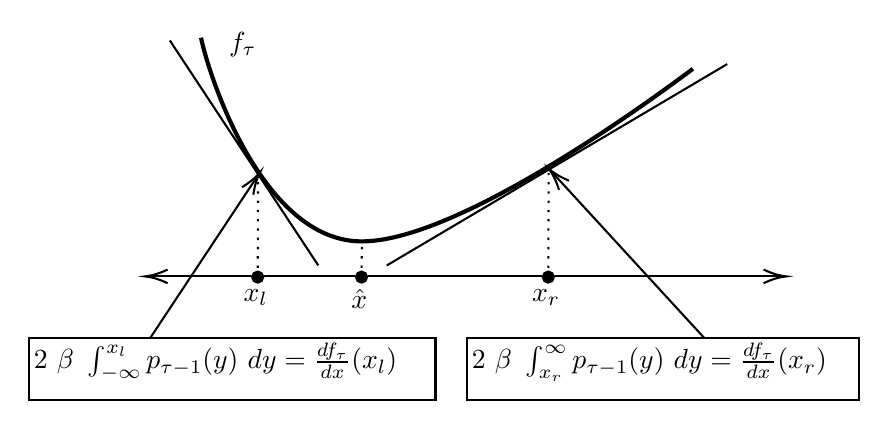
\begin{tikzpicture}[x=0.75pt,y=0.75pt,yscale=-1,xscale=1]
%uncomment if require: \path (0,308); %set diagram left start at 0, and has height of 308

%Curve Lines [id:da37061921880533877] 
\draw [line width=1.5]    (98,85.33) .. controls (102.36,105.81) and (127.25,179.72) .. (172,183.33) .. controls (216.75,186.95) and (312.43,117.26) .. (335,100.33) ;
%Straight Lines [id:da8132100594867722] 
\draw    (73,200.33) -- (378,200.33) ;
\draw [shift={(380,200.33)}, rotate = 180] [color={rgb, 255:red, 0; green, 0; blue, 0 }  ][line width=0.75]    (10.93,-3.29) .. controls (6.95,-1.4) and (3.31,-0.3) .. (0,0) .. controls (3.31,0.3) and (6.95,1.4) .. (10.93,3.29)   ;
\draw [shift={(71,200.33)}, rotate = 0] [color={rgb, 255:red, 0; green, 0; blue, 0 }  ][line width=0.75]    (10.93,-3.29) .. controls (6.95,-1.4) and (3.31,-0.3) .. (0,0) .. controls (3.31,0.3) and (6.95,1.4) .. (10.93,3.29)   ;
%Shape: Circle [id:dp2801837798690885] 
\draw  [fill={rgb, 255:red, 0; green, 0; blue, 0 }  ,fill opacity=1 ] (172.67,200.67) .. controls (172.67,199.19) and (173.86,198) .. (175.33,198) .. controls (176.81,198) and (178,199.19) .. (178,200.67) .. controls (178,202.14) and (176.81,203.33) .. (175.33,203.33) .. controls (173.86,203.33) and (172.67,202.14) .. (172.67,200.67) -- cycle ;
%Shape: Circle [id:dp9237316574850754] 
\draw  [fill={rgb, 255:red, 0; green, 0; blue, 0 }  ,fill opacity=1 ] (262.67,200.67) .. controls (262.67,199.19) and (263.86,198) .. (265.33,198) .. controls (266.81,198) and (268,199.19) .. (268,200.67) .. controls (268,202.14) and (266.81,203.33) .. (265.33,203.33) .. controls (263.86,203.33) and (262.67,202.14) .. (262.67,200.67) -- cycle ;
%Shape: Circle [id:dp045787056716331875] 
\draw  [fill={rgb, 255:red, 0; green, 0; blue, 0 }  ,fill opacity=1 ] (122.67,200.67) .. controls (122.67,199.19) and (123.86,198) .. (125.33,198) .. controls (126.81,198) and (128,199.19) .. (128,200.67) .. controls (128,202.14) and (126.81,203.33) .. (125.33,203.33) .. controls (123.86,203.33) and (122.67,202.14) .. (122.67,200.67) -- cycle ;
%Straight Lines [id:da08221456294078888] 
\draw    (83,86.67) -- (154.52,195.05) ;
%Straight Lines [id:da4107386957452337] 
\draw    (351.52,98.05) -- (187.52,195.05) ;
%Straight Lines [id:da4276666085658716] 
\draw  [dash pattern={on 0.84pt off 2.51pt}]  (125.33,200.67) -- (125.52,149.05) ;
%Straight Lines [id:da6234026284865279] 
\draw  [dash pattern={on 0.84pt off 2.51pt}]  (265.33,200.67) -- (265.52,146.38) ;
%Straight Lines [id:da7796663876642187] 
\draw  [dash pattern={on 0.84pt off 2.51pt}]  (175.33,200.67) -- (175.52,184.05) ;
%Straight Lines [id:da05642327969494221] 
\draw    (73.52,230.05) -- (125.42,151.71) ;
\draw [shift={(126.52,150.05)}, rotate = 483.52] [color={rgb, 255:red, 0; green, 0; blue, 0 }  ][line width=0.75]    (10.93,-3.29) .. controls (6.95,-1.4) and (3.31,-0.3) .. (0,0) .. controls (3.31,0.3) and (6.95,1.4) .. (10.93,3.29)   ;
%Straight Lines [id:da7628684000665404] 
\draw    (340.52,230.05) -- (266.88,149.85) ;
\draw [shift={(265.52,148.38)}, rotate = 407.44] [color={rgb, 255:red, 0; green, 0; blue, 0 }  ][line width=0.75]    (10.93,-3.29) .. controls (6.95,-1.4) and (3.31,-0.3) .. (0,0) .. controls (3.31,0.3) and (6.95,1.4) .. (10.93,3.29)   ;

% Text Node
\draw (169,205) node [anchor=north west][inner sep=0.75pt]    {$\hat{x}$};
% Text Node
\draw (117,205) node [anchor=north west][inner sep=0.75pt]    {$x_{l}$};
% Text Node
\draw (256,205) node [anchor=north west][inner sep=0.75pt]    {$x_{r}$};
% Text Node
\draw  [fill={rgb, 255:red, 255; green, 255; blue, 255 }  ,fill opacity=1 ]  (15,230) -- (211,230) -- (211,260) -- (15,260) -- cycle  ;
\draw (16,231) node [anchor=north west][inner sep=0.75pt]    {$2\ \beta \ \int _{-\infty }^{x_{l}} p_{\tau -1}( y) \ dy=\frac{df_{\tau }}{dx}( x_{l})$};
% Text Node
\draw (110,81) node [anchor=north west][inner sep=0.75pt]    {$f_{\tau }$};
% Text Node
\draw  [fill={rgb, 255:red, 255; green, 255; blue, 255 }  ,fill opacity=1 ]  (226,230) -- (415,230) -- (415,260) -- (226,260) -- cycle  ;
\draw (227,231) node [anchor=north west][inner sep=0.75pt]    {$2\ \beta \ \int _{x_{r}}^{\infty } p_{\tau -1}( y) \ dy=\frac{df_{\tau }}{dx}( x_{r})$};


\end{tikzpicture}

    \caption{Visualization of the choice of $x_l$ and $x_r$ of the probabilistic algorithm.}
    \label{fig:probabilistic_algorithm}
\end{figure}

\paragraph{Root Finding} The previous arguments show that a bracketed root finding method can be used to find $x_l$ and $x_r$. We use \emph{Brent's method}\index{Brent's method} for root finding. Brent's method combines the bisection method with higher-order methods to guarantee convergence to the root, yet at a higher rate than if only bisection were used~\cite{Press2007}. \citeauthor*{Press2007}~\cite{Press2007} ``recommend it as the method of choice for general one-dimensional
root finding where a function’s values only (and not its derivative or functional form)
are available''. We denote the convergence rate of approximating the root with tolerance $\epsilon$ by $\mathcal{O}(R_{\epsilon})$.

\paragraph{Numerical Differentiation} We use the \emph{five-point stencil}\index{five-point stencil} \begin{align*}
    \diff{f_{\tau}}{x}(x) \approx \frac{-f_{\tau}(x - 2h) + 8 f_{\tau}(x + h) - 8 f_{\tau}(x - h) + f_{\tau}(x - 2h)}{12h}
\end{align*} to find a finite difference approximation of order $\mathcal{O}(h)$ of the first order derivative of $f_{\tau}$ at configurations $x \in \mathcal{X}$~\cite{Sauer2011}. To match the accuracy of our convex optimizations we set $h := \epsilon / 10$. To approximate the second order derivative of $f_{\tau}$ at a configuration $x \in \mathcal{X}$ we use \begin{align*}
    \diff[2]{f_{\tau}}{x}(x) \approx \frac{-f_{\tau}(x + 2h) + 16 f_{\tau}(x+h) - 30 f_{\tau}(x) + 16 f_{\tau}(x-h) - f_{\tau}(x - 2h)}{12 h^2}
\end{align*} which yields an approximation of order $\mathcal{O}(h^4)$~\cite{Sauer2011}. Thus, we set $h := (\epsilon / 10)^{-1/4}$. We are thus able to compute these approximations in $\mathcal{O}(C)$ time.

Next, we describe how the constraints from \cref{eq:ud:probabilistic:right} and \cref{eq:ud:probabilistic:left} can be computed numerically.

\paragraph{Numerical Integration} In our implementation, we need to compute both finite and semi-infinite integrals over the probability distribution $p$.

We use the \emph{Tanh-sinh quadrature}\index{Tanh-sinh quadrature} (also known as the double exponential method) to compute finite integrals. \citeauthor*{Bailey2005}~\cite{Bailey2005} describe the convergence and error of this method in more detail. They conclude that ``overall, the tanh-sinh scheme appears to be the best
for integrands of the type most often encountered in experimental math research'' and highlight that it has ``excellent accuracy and runtime performance''~\cite{Bailey2005}.

We use the \emph{Gauss-Laguerre quadrature}\index{Gauss-Laguerre quadrature} for semi-infinite integrals, which approximates values of integrals of the kind \begin{align}\label{eq:gauss_laguerre}
    \int_0^{\infty} e^{-x} f(x) \,dx
\end{align}~\cite{Weisstein}. It is easy to see that we can eliminate the weights by multiplying the integrand $g$ with $e^x$. Let $\text{GL}(g)$ denote the approximation of \cref{eq:gauss_laguerre} obtained by the Gauss-Laguerre quadrature. We are then able to compute any right-open integral over the interval $[{a,\infty})$ with integrand $p$ by setting $g(x) := p(a+x)$ and any left-open integral over the interval $({-\infty,b}]$ with integrand $p$ by setting $g(x) := p(b-x)$.

Crucially, for numeric stability in both integration schemes, we need that the integrands are continuous. It is easy to see that, in general, this is not the case for our probability distribution $p$. We describe in the following paragraph how integrals can be suitably discretized to allow for stable numeric results. Moreover, as the integration schemes are not universal, probability distributions exist for which the used quadratures cannot find the integral. In such a case, one would have to resort to another integration scheme. We denote the convergence rate of approximating the integral with tolerance $\epsilon$ by $\mathcal{O}(I_{\epsilon})$.

\paragraph{Piecewise Linear Hitting Costs} We have already discharged the assumptions that $\beta = 1$ and that the decision space is unbounded. It remains to extend this algorithm to allow for piecewise linear hitting costs.

In our description of the adaption to piecewise linear hitting costs $f_{\tau}$, we refer to the non-continuous or non-smooth points of $f_{\tau}$ as \emph{breakpoints}\index{breakpoint}. For a piecewise linear function, we can discretize the integral into a summation, replace the first-order derivative at a breakpoint by the difference of consecutive points, and replace the second-order derivative at a point by the difference in slopes of consecutive points~\cite{Bansal2015}. Let $B_{f_{\tau}}$ denote the set of breakpoints of $f_{\tau}$. Further, we denote by $x_{\tau,l}$ and $x_{\tau,r}$ the values of $x_l$ and $x_r$ at time $\tau$, respectively. It is easy to see that the set of breakpoints of $p_{\tau}$ is then given by \begin{align*}
    B_{p_{\tau}} := \{0, m\} \cup \left(B_{f_1} \cup \{x_{1,l}, x_{1,r}\}\right) \cup \dots \cup \left(B_{f_{\tau}} \cup \{x_{\tau,l}, x_{\tau,r}\}\right).
\end{align*}

Let $B_{p_{\tau}}^I := B_{p_{\tau}} \cap I$. The integral of $p_{\tau}$ over $I \subseteq \mathbb{R} \cup \{-\infty, \infty\}$ can then be computed using the quadrature methods described previously by integrating piecewise: \begin{align*}
    \int_I p_{\tau}(y) \,dy = \int_{\min I}^{\min B_{p_{\tau}}^I} p_{\tau}(y) \,dy + \int_{\max B_{p_{\tau}}^I}^{\max I} p_{\tau}(y) \,dy + \sum_{(i, j) \in \text{sort}(B_{p_{\tau}}^I)} \int_i^j p_{\tau}(y) \,dy
\end{align*} where $\text{sort}(A)$ denotes the pairs of consecutive elements of some set $A \subset \mathbb{R}$ in ascending order. We can continue to use finite difference approximations for the first-order and second-order derivatives.

\paragraph{} Note that the computation of $p_{\tau}$ requires $\mathcal{O}(\tau)$ many approximations of the second-order derivative of $f_{t}$. Therefore, any evaluation of $p_{\tau}$ requires $\mathcal{O}(\tau C)$ time and we are thus able to compute the $\epsilon$-optimal integral in $\mathcal{O}(\tau C I_{\epsilon} |B_{p_{\tau}}|) = \mathcal{O}(\tau^2 C I_{\epsilon} |B_{f_0}|)$ time, assuming $B_{f_{\tau}}$ add a constant number of new breakpoints in each time step and with $B_{f_0}$ denoting the number of breakpoints that is shared between multiple $f_{\tau}$. Overall, the described convex optimizations can be solved $\epsilon$-optimally in $\mathcal{O}(\tau^2 C I_{\epsilon} |B_{f_0}| R_{\epsilon} O_{\epsilon}^1)$ time. This is also the time complexity of the algorithm. This shows that, similarly to lazy capacity provisioning, the computational complexity grows polynomially with time. However, unlike lazy capacity provisioning, we cannot regularly reset the history, rendering this algorithm computationally inefficient for short time slot lengths. The algorithm is described in \cref{alg:ud:probabilistic}.

\begin{algorithm}
    \caption{Probabilistic algorithm~\cite{Bansal2015}}\label{alg:ud:probabilistic}
    \SetKwInOut{Input}{Input}
    \Input{$\mathcal{I}_{\text{SSCO}} = (\tau \in \mathbb{N}, m \in \mathbb{N}, \beta \in \mathbb{R}_{>0}, (f_1, \dots, f_{\tau}) \in (\mathbb{R}_{\geq 0} \to \mathbb{R}_{\geq 0})^{\tau})$}
    $\hat{x} \gets \argmin_{x \in \mathcal{X}} f_{\tau}(x)$\;
    find $x_r$ using the optimization described by \cref{eq:ud:probabilistic:right} subject to $x \in \mathcal{X}$\;
    find $x_l$ using the optimization described by \cref{eq:ud:probabilistic:left} subject to $x \in \mathcal{X}$\;
    set $p_{\tau}$ based on the update rule in \cref{eq:ud:probabilistic:update}\;
    \Return $\int_{x_l}^{x_r} y \cdot p_{\tau}(y) \,dy$\;
\end{algorithm}

Updating the probability distribution $p$ can be done in constant time as this does not require any function evaluations. As discussed in the beginning of this subsection, given a uniformly picked $\gamma \in [0,1]$, the randomized algorithm chooses $X_{\tau}$ (randomly) such that $\int_{-\infty}^{X_{\tau}} p_{\tau}(y) \,dy = \gamma$. In other words, $P_{\tau}(X_{\tau}) \sim \text{Unif}(0,1)$ where $P_{\tau}$ is the cumulative distribution function of $p_{\tau}$. By the universality of the uniform, $X_{\tau}$ is $P_{\tau}$-distributed, i.e. $X_{\tau} \sim P_{\tau}$. Hence, $E X_{\tau} = \int_{x_l}^{x_r} y \cdot p_{\tau}(y) \,dy$ computes the configuration for time slot $\tau$ as $p_{\tau}(y) = 0$ for $y \not\in [x_l, x_r]$. We then return $E X_{\tau}$. Similarly to the previously discussed integrals, this integral can be computed $\epsilon$-optimally in $\mathcal{O}(\tau^2 C I_{\epsilon} |B_{f_0}|)$ time, not affecting the asymptotic time complexity of the algorithm.

\subsection{Randomly Biased Greedy Algorithm}\label{section:online_algorithms:ud:rbg}

We have seen many constant-competitive online algorithms for uni-dimensional smoothed convex optimization. However, we have not yet paid much attention to minimizing regret. This is also partially because sublinear regret can be achieved easily using online gradient descent. As this approach generalizes to the multi-dimensional setting, we discuss this approach in \cref{section:online_algorithms:md:descent_methods} more generally looking at descent methods.

Still, one important question regarding the uni-dimensional setting remains, namely, whether there is an algorithmic framework that achieves both a constant-competitive ratio and sublinear regret. While it is impossible to achieve both simultaneously, it is possible to develop an algorithmic framework that balances both performance metrics.

In their paper, where the incompatibility between the competitive ratio and regret was first introduced, \citeauthor*{Andrew2015}~\cite{Andrew2015} already proposed an algorithmic framework for SCO balancing the two notions in the uni-dimensional setting. Their approach is to scale the norm used to penalize movement in the decision space with a parameter $\theta \geq 1$. If $\theta = 1$, i.e., the algorithm solves the original problem, their algorithm is $2$-competitive and has linear regret. In contrast, for $\theta > 1$, movement in the decision space is penalized more. This allows reducing the regret to an arbitrary amount (which still depends linearly on $T$) while maintaining a constant competitive ratio~\cite{Andrew2015}.

Note that while regret is understood as introduced in \cref{section:theory:performance_metrics}, the competitive ratio is understood with respect to the modified problem with lookahead $1$. In general, with \emph{lookahead}\index{lookahead} $i$, the environment plays actions $i$ steps before the agent follows suit. In other words, a step at time $i$ is evaluated using the cost function from time $t-i$, and the initial step $X_i$ is $\mathbf{0}$. For lookahead $i$, we consider the modified overall cost \begin{align*}
    \sum_{t=1}^T f_t(X_{t+i}) + \norm{X_{t+i} - X_{t+i-1}}.
\end{align*} For $i=1$, this modified problem is equivalent to metrical task systems where the environment plays first. In contrast, with SCO, the agent plays first, resulting in a lookahead of $i=0$~\cite{Andrew2015}. Note that SCO is the more restricted setting as the agent has less knowledge than in metrical task systems implying that the corresponding competitive algorithm for lookahead $0$ is as competitive as the discussed algorithm for lookahead $i$. Given an algorithm with lookahead $i$, the corresponding algorithm with lookahead $0$ is obtained simply by shifting determined configurations $i$ time slots into the past.

\citeauthor*{Bansal2015}~\cite{Bansal2015} mention in their paper that the claims on this algorithm were withdrawn, however, \citeauthor*{Andrew2015}~\cite{Andrew2015} clarified their proof, showing it is correct as stated in the original paper~\cite{Wierman}.

The algorithm of \citeauthor*{Andrew2015}~\cite{Andrew2015} is initialized with a random parameter $r$ which is uniformly sampled from $({-1,1})$, i.e. $r \sim \text{Unif}(-1, 1)$. They define the work function \begin{align}\label{eq:randomly_biased_greedy:work_function}
    w_{\tau}(x) = \min_{y \in \mathcal{X}} w_{\tau-1}(y) + f_{\tau}(y) + \theta \norm{x - y}
\end{align} where $w_0(x) = \theta \norm{x}$. During each time slot $\tau$ the algorithm moves to the configuration $x$ minimizing $w_{\tau-1}(x) + r \theta \norm{x}$. The resulting algorithm is described in \cref{alg:ud:rbg}.

\begin{algorithm}
    \caption{Randomly Biased Greedy~\cite{Andrew2015}}\label{alg:ud:rbg}
    \SetKwInOut{Input}{Input}
    \Input{$\mathcal{I}_{\text{SCO}} = (\tau \in \mathbb{N}, \mathcal{X} \subset \mathbb{R}, \norm{\cdot}, (f_1, \dots, f_{\tau}) \in (\mathcal{X} \to \mathbb{R}_{\geq 0})^{\tau}), \theta \geq 1, r \sim \text{Unif}(-1,1)$}
    $x \gets \argmin_{x \in \mathcal{X}} w_{\tau-1}(x) + r \theta \norm{x}$\;
    set $w_{\tau}$ as described in \cref{eq:randomly_biased_greedy:work_function}\;
    \Return $x$\;
\end{algorithm}

Observe that as expected, the algorithm returns $X_1 = \mathbf{0}$ for the initial step.

\citeauthor*{Andrew2015}~\cite{Andrew2015} show that given a $\theta \geq 1$ their algorithm attains the $\alpha$-unfair competitive ratio $(1+\theta) / \min \{\theta, \alpha\}$ and regret $\mathcal{O}(\max \{T / \theta, \theta\})$. Hence, for $\alpha = 1$ and $\theta = 1$ the algorithm is $2$-competitive. For any $\alpha > 0$, the optimal $\alpha$-unfair competitive ration is $1 + 1 / \alpha$ and obtained by setting $\theta = \alpha$. In contrast, $\theta = 1 / \epsilon$ for some $\epsilon > 0$ yields the minimal regret $\mathcal{O}(\epsilon T)$~\cite{Andrew2015}. In general, when $T$ is known in advance, \citeauthor*{Andrew2015}~\cite{Andrew2015} show that for $\theta \in \mathcal{O}(\sqrt{T})$, their algorithm achieves a $\mathcal{O}(\sqrt{T})$ $\alpha$-unfair competitive ratio and $\mathcal{O}(\sqrt{T})$ regret.

It is easy to see that the work function itself is convex as it can be interpreted as the inf-projection of the convex function $f(x,y) = w_{\tau-1}(y) + f_{\tau}(y) + \theta \norm{x - y}$. This fact is shown in proposition 2.22 of~\cite{Burke2015}. The evaluation of $w_{\tau}$ requires $\mathcal{O}(\tau)$ recursive evaluations of the work function each of which uses a convex optimization and evaluates the hitting costs. Thus, an $\epsilon$-optimal evaluation of $w_{\tau}$ can be obtained in $\mathcal{O}(C (O_{\epsilon}^1)^{\tau})$ time. Hence, the overall time complexity of the algorithm is in $\mathcal{O}(C (O_{\epsilon}^1)^{\tau+1})$. We improve the practical runtime by memoizing the work function.

\subsection{Randomized Integral Relaxation}

\citeauthor*{Albers2018}~\cite{Albers2018} use the probabilistic algorithm described in \cref{section:online_algorithms:ud:probabilistic} in their randomized algorithm for Int-SSCO achieving the optimal competitive ratio $2$ against an oblivious adversary. Although they used the probabilistic algorithm in their paper, their proof generalizes to any $2$-competitive fractional algorithm, so, in particular, the randomly biased greedy algorithm can be used as well. Roughly, the algorithm works by solving the relaxed problem using the probabilistic algorithm of \citeauthor*{Bansal2015}~\cite{Bansal2015} and then randomly rounding the resulting fractional schedule.

Let $\bar{\mathcal{I}} = (T, m, \beta, \bar{F})$ with $\bar{F} = (\bar{f}_1, \dots, \bar{f}_T)$ be the fractional relaxation of the instance $\mathcal{I} = (T, m, \beta, F)$ of Int-SSCO and let $\bar{\mathcal{X}} = [0,m]$ denote the decision space of $\bar{\mathcal{I}}$. \citeauthor*{Albers2018}~\cite{Albers2018} define the relaxed operating costs $\bar{f}_{\tau} : \bar{\mathcal{X}} \to \mathbb{R}_{\geq 0}$ as the linear interpolation of the integral operating costs $f_{\tau}$: \begin{align*}
    \bar{f}_{\tau} := \begin{cases}
        f_{\tau}(x) & x \in [m]_0 \\
        (\lceil x \rceil - x) f_{\tau}(\lfloor x \rfloor) + (x - \lfloor x \rfloor) f_{\tau}(\lceil x \rceil) & \text{otherwise}.
    \end{cases}
\end{align*} Note that $\bar{f_{\tau}}$ are continuous and piecewise linear with the set of breakpoints $[m]_0$. Hence, we are able to use \cref{alg:ud:probabilistic} to obtain the configuration $\bar{X}_{\tau} \in \bar{\mathcal{X}}$ at time $\tau$ for the relaxed problem instance  $\bar{\mathcal{I}}$. Further, let $\text{frac}(x) = x - \lfloor x \rfloor$ be the fractional part of $x$ and let $\bar{X}'_{\tau-1} = (\bar{X}_{\tau-1})_{\lfloor\bar{X}_{\tau}\rfloor}^{\lceil\bar{X}_{\tau}\rceil}$ be the projection of the preceding relaxed configuration onto the discrete interval of the current relaxed configuration.

The randomized algorithm distinguishes between time slots where the configuration is increased and time slots where the configuration is decreased. In the first case, i.e. $\bar{X}_{\tau-1} \leq \bar{X}_{\tau}$, if $X_{\tau-1} = \lceil\bar{X}_{\tau}\rceil$  the configuration remains unchanged. Otherwise, $X_{\tau}$ is set to $\lceil\bar{X}_{\tau}\rceil$ with probability \begin{align*}
    p_{\tau}^{\uparrow} := \frac{\bar{X}_{\tau} - \bar{X}'_{\tau-1}}{1 - \text{frac}(\bar{X}'_{\tau-1})}
\end{align*} and to $\lfloor\bar{X}_{\tau}\rfloor$ with probability $1 - p_{\tau}^{\uparrow}$. Conversely, if $\bar{X}_{\tau-1} > \bar{X}_{\tau}$, the configuration remains unchanged if $X_{\tau-1} = \lfloor\bar{X}_{\tau}\rfloor$, and otherwise with probability \begin{align*}
    p_{\tau}^{\downarrow} := \frac{\bar{X}'_{\tau-1} - \bar{X}_{\tau}}{\text{frac}(\bar{X}'_{\tau-1})}
\end{align*} the configuration is set to $\lfloor\bar{X}_{\tau}\rfloor$ and with probability $p_{\tau}^{\downarrow}$ the configuration is set to $\lceil\bar{X}_{\tau}\rceil$. The resulting algorithm is shown in \cref{alg:ud:randomized}.

\begin{algorithm}
    \caption{Randomized integral relaxation~\cite{Albers2018}}\label{alg:ud:randomized}
    \SetKwInOut{Input}{Input}
    \Input{$\mathcal{I}_{\text{Int-SSCO}} = (\tau \in \mathbb{N}, m \in \mathbb{N}, \beta \in \mathbb{R}_{>0}, (f_1, \dots, f_{\tau}) \in (\mathbb{N}_0 \to \mathbb{R}_{\geq 0})^{\tau})$}
    $\bar{X}_{\tau} \gets \text{\cref{alg:ud:probabilistic}}(\bar{\mathcal{I}}_{\text{Int-SSCO}})$\;
    \eIf{$\bar{X}_{\tau-1} \leq \bar{X}_{\tau}$}{
        \eIf{$X_{\tau-1} = \lceil\bar{X}_{\tau}\rceil$}{
            \Return $\lceil\bar{X}_{\tau}\rceil$\;
        }{
            $\gamma \sim \text{Unif}(0,1)$\;
            \eIf{$\gamma \leq p_{\tau}^{\uparrow}$}{
                \Return $\lceil\bar{X}_{\tau}\rceil$\;
            }{
                \Return $\lfloor\bar{X}_{\tau}\rfloor$\;
            }
        }
    }{
        \eIf{$X_{\tau-1} = \lfloor\bar{X}_{\tau}\rfloor$}{
            \Return $\lfloor\bar{X}_{\tau}\rfloor$\;
        }{
            $\gamma \sim \text{Unif}(0,1)$\;
            \eIf{$\gamma \leq p_{\tau}^{\downarrow}$}{
                \Return $\lfloor\bar{X}_{\tau}\rfloor$\;
            }{
                \Return $\lceil\bar{X}_{\tau}\rceil$\;
            }
        }
    }
\end{algorithm}

We use the universality of the uniform to simulate Bernoulli-distributed random variables with parameters $p_{\tau}^{\uparrow}$ and $p_{\tau}^{\downarrow}$, respectively. Any pseudo-random number generator can be used to produce the uniformly distributed $\gamma$. It is easy to see that the time complexity is given by the time complexity of \cref{alg:ud:probabilistic}, i.e., $\mathcal{O}(\tau^2 m C I_{\epsilon} R_{\epsilon} O_{\epsilon}^1)$ with $|B_{f_0}| \in \mathcal{O}(m)$, or the complexity of \cref{alg:ud:rbg}, i.e., $\mathcal{O}(C (O_{\epsilon}^1)^{\tau+1})$ depending on which algorithm is used for the relaxed problem.

\section{Multi-Dimensional}\label{section:online_algorithms:md}

\subsection{Lazy Budgeting}\label{section:online_algorithms:md:lazy_budgeting}

To begin with our discussion of the multi-dimensional setting, we examine two algorithms developed by \citeauthor*{Albers2021}~\cite{Albers2021} for a restricted class of convex cost functions. Their first algorithm is $2d$-competitive for SLO, i.e., load and time-independent costs, and their second algorithm is $(2d+1)$-competitive for SBLO. Note that we only defined SBLO and SLO for the integral case. As no online algorithm for SLO can attain a competitive ratio smaller than $2d$, their first algorithm is optimal, and their second algorithm is nearly optimal~\cite{Albers2021, Albers2021_2}.

The idea behind both algorithms is to calculate optimal schedules up to the current time slot. Depending on this schedule, the algorithm decides if a server is powered up. To perform the smoothing, the algorithm remembers how long a server was idling and powers this server down if the idle duration surpasses a threshold. \citeauthor*{Albers2021}~\cite{Albers2021} do not name their algorithms, yet, within this work, we refer to them as \emph{lazy budgeting methods}\index{lazy budgeting}.

\subsubsection{Lazy Budgeting for Smoothed Load Optimization}

Let $\mathcal{I} = (d, \tau, m, \beta, \Lambda, c)$ be an instance of SLO. \citeauthor*{Albers2021}~\cite{Albers2021} focus on a setting without inefficient server types. A server type $k$ is called \emph{inefficient} if there exists another server type $k'$ where both the operating cost and the switching cost is lower, i.e. $c_k \geq c_{k'}$ and $\beta_k \geq \beta_{k'}$. In practice, this is not a restriction as a server of an inefficient server type is only ever powered up if all more efficient servers are already active as there is no trade-off between operating and switching costs. Furthermore, typically servers with a lower operating cost also have a higher switching cost. In addition, \citeauthor*{Albers2021} assume that there are no duplicated server types, i.e., server types with equal operating and switching costs.

We assume that the server types are sorted in descending order by their operating costs, i.e. $c_1 > \dots > c_d$. As we excluded inefficient server types, switching costs are in ascending order, $\beta_1 < \dots < \beta_d$.

The algorithm of \citeauthor*{Albers2021}~\cite{Albers2021} separates a problem instance into $m := \sum_{k=1}^d m_k$ lanes. Recall that with SLO, we assume that each active server can handle a single job during each time slot. The algorithm uses that at time slot $t$ there is a job in line $j$ if and only if $j \leq \lambda_{t}$. Thus, all servers represented by lines $j > \lambda_{t}$ are either inactive or idling.

Let $y_{t,j}$ denote the server type that handles the $j$-th lane during time slot $t$ given some underlying schedule $X$. We say $y_{t,j} = 0$ if there is no active server in lane $j$ during time slot $t$, which is only the case if $j > \lambda_{t}$ as we can assume that $\lambda_{t} \leq m$ holds for all time slots $t \in [T]$. \citeauthor*{Albers2021}~\cite{Albers2021} give the following formal definition: \begin{align*}
    y_{t,j} := \begin{cases}
        \max \{k \in [d] \mid \sum_{k' = k}^d X_{t,k'} \geq j\} & k \in \left[\sum_{k=1}^d X_{t,k}\right] \\
        0 & \text{otherwise}.
    \end{cases}
\end{align*} By this definition, we prefer to use servers of the server type with the lowest operating cost (and largest switching cost). In other words, the server types handling each lane $y_{t,1}, \dots, y_{t,m}$ are sorted in descending order, i.e. $y_{t,j} \geq y_{t,j'}$ for $j < j'$. We denote by $\hat{y}_{t,j}^{\tau}$ the server type in lane $j$ during time slot $t$ induced by some optimal schedule $\hat{X}^{\tau}$ up to time $\tau$ and by $\widetilde{y}_{t,j}$ the server type in lane $j$ during time slot $t$ as assigned by the algorithm.

The algorithm begins by finding an optimal schedule $\hat{X}^{\tau}$ up to time slot $\tau$. This schedule is chosen such that the server type in a lane of $\hat{X}^{\tau}$ is never reduced compared to the previously used optimal schedule $\hat{X}^{\tau-1}$, i.e. $\hat{y}_{t,j}^{\tau} \geq \hat{y}_{t,j}^{\tau-1}$ for all time slots $t \in [\tau]$ and lanes $j \in [m]$. Moreover, we assume that $\hat{X}^{\tau}$ is a schedule that powers up servers as late as possible and powers down servers as early as possible. This is necessary in case $c_k = 0$ for some server type $k \in [d]$. We observe that these properties are fulfilled by all optimal schedules that \cref{alg:md:optimal_graph_search} obtains. We cache the results of the optimal graph-based algorithm such that in every iteration of the online algorithm, only one dynamic update needs to be performed. The asymptotic time complexity of this dynamic update is thus given as $\mathcal{O}(|\mathcal{M}| C d)$ where $|\mathcal{M}| \in \mathcal{O}(\prod_{k=1}^d m_k)$.

Now, the algorithm ensures that no server type is used for lane $j \in [m]$ that is smaller than the server type used by $\hat{X}^{\tau}$, i.e. $\widetilde{y}_{\tau,j} \geq \hat{y}_{\tau,j}^{\tau}$. If $\widetilde{y}_{\tau-1,j} < \hat{y}_{\tau,j}^{\tau}$, a server of type $\widetilde{y}_{\tau-1,j}$ is powered down and a server of type $\hat{y}_{\tau,j}^{\tau}$ is powered up. A server of type $k$ that is not replaced by a greater server type remains active for $\bar{t}_k := \lfloor \beta_k / c_k \rfloor$ time slots~\cite{Albers2021}. If $\hat{X}^{\tau}$ uses a smaller server type $k' \leq k$ in the meantime, then the server of type $k$ will run for at least $\bar{t}_{k'}$ further time slots.

The algorithm computes $\widetilde{y}_{\tau,j}$ directly. The corresponding number of active servers of type $k$ of the underlying schedule $\widetilde{X}$ can be obtained by $\widetilde{X}_{\tau,j} = |\{j \in [m] \mid \widetilde{y}_{\tau,j} = k\}|$. The resulting algorithm is shown in \cref{alg:md:lazy_budgeting:det_slo}. Here, $h_j$ denotes the time until the server handling line $j \in [m]$ is powered down.

\begin{algorithm}
    \caption{Lazy Budgeting for SLO~\cite{Albers2021}}\label{alg:md:lazy_budgeting:det_slo}
    \KwIn{$\mathcal{I}_{\text{SLO}} = (d \in \mathbb{N}, \tau \in \mathbb{N}, m \in \mathbb{N}^d, \beta \in \mathbb{R}_{>0}^d, \Lambda \in \mathbb{N}_0^{\tau}, c \in \mathbb{R}_{\geq 0}^d)$}
    Update the previously found optimal schedule $\hat{X}^{\tau-1}$ to $\hat{X}^{\tau}$ such that $\hat{y}_{t,j}^{\tau} \geq \hat{y}_{t,j}^{\tau-1}$ for all  $j \in [m]$\;
    \For{$j \gets 1$ \KwTo $m$}{
        \eIf{$\widetilde{y}_{\tau-1,j} < \hat{y}_{\tau,j}^{\tau}$ \KwOr $t \geq h_j$}{
            $\widetilde{y}_{\tau,j} \gets \hat{y}_{\tau,j}^{\tau}$\;
            $h_j \gets \tau + \bar{t}_{\hat{y}_{\tau,j}^{\tau}}$\;
        }{
            $\widetilde{y}_{\tau,j} \gets \widetilde{y}_{\tau-1,j}$\;
            $h_j \gets \max \{h_j, \tau + \bar{t}_{\hat{y}_{\tau,j}^{\tau}}\}$ where $\bar{t}_0 = 0$\;
        }
    }
    \ForEach{$k \in [d]$}{
        $X_{\tau,k} \gets |\{j \in [m] \mid \widetilde{y}_{\tau,j} = k\}|$\;
    }
    \Return $X_{\tau}$\;
\end{algorithm}

\begin{function}
	\caption{BuildLanes($x, d, m$)}\label{proc:md:lazy_budgeting:build_lanes}
	$y \gets \mathbf{0}$\;
	\For{$j \gets 1$ \KwTo $m$}{
	    \If{$j \leq \sum_{k=1}^d x_k$}{
	        \For{$k \gets 1$ \KwTo $d$}{
        	    \If{$\sum_{k'=k}^d x_{k'} \geq j$}{
        	        $y_j \gets k$\;
        	    }
        	}
	    }
	}
    \Return $y$\;
\end{function}

Schedules can be converted to lanes in $\mathcal{O}(m d^2)$ time as described by \ref{proc:md:lazy_budgeting:build_lanes} and lanes can be converted back to schedules in $\mathcal{O}(m)$ time by iterating over all lanes. Hence, the overall asymptotic time complexity of the algorithm is described by adding the time required to find the optimal schedule, i.e., $\mathcal{O}(m d^2 + C d \prod_{k=1}^d m_k)$.

\subsubsection{Randomized Lazy Budgeting for Smoothed Load Optimization}

\citeauthor*{Albers2021}~\cite{Albers2021} describe how the competitive ratio of the previously described \cref{alg:md:lazy_budgeting:det_slo} can be improved to $\frac{e}{e-1}d \approx 1.582d$ against an oblivious adversary by randomizing the running time of a server. Before execution, the randomized algorithm chooses $\gamma \in [0,1]$ according to the probability density function \begin{align*}
    f_{\gamma}(x) = \begin{cases}
        e^x / (e-1) & x \in [0,1] \\
        0 & \text{otherwise}.
    \end{cases}
\end{align*} Then, the running time of a server of type $k \in [d]$, $\bar{t}_k$, is set to $\lfloor \gamma \cdot \beta_k / c_k \rfloor$.

To sample $\gamma$ we first seek to find the cumulative distribution function $F_{\gamma}$. For $x \in [0,1]$ we have \begin{align*}
    F_{\gamma}(x) &= \int_0^x f_{\gamma}(t) \,dt \\
                  &= \frac{1}{e-1} \int_0^x e^t \,dt \\
                  &= \frac{1}{e-1} (e^x - 1).
\end{align*} By the universality of the uniform, realizations of $F_{\gamma}$ can be simulated given $U \sim \text{Unif}(0,1)$ as $F_{\gamma}^{-1}(U) \sim F_{\gamma}$. It is now easy to see that $F_{\gamma}^{-1}(x) = \ln (x (e - 1) + 1)$.

This completes the description of the implementation of the randomized variant of lazy budgeting for SLO. The asymptotic time complexity is given by the time complexity of \cref{alg:md:lazy_budgeting:det_slo}.

\subsubsection{Lazy Budgeting for Smoothed Balanced-Load Optimization}

In a subsequent paper, \citeauthor*{Albers2021_2}~\cite{Albers2021_2} modified their lazy budgeting method to SBLO, allowing for more complex cost functions. The method remains similar: First, an optimal schedule is found which ends at the current time slot. Then, the algorithm ensures for each server type that the number of active servers is at least as large as the number of active servers in the optimal schedule. Lastly, to make the algorithm competitive, if the accumulated idle operating cost of a server of type $k$, $g_{t,k}(0)$ exceeds the switching cost $\beta_k$, a server of type $k$ is powered down.

First, \citeauthor*{Albers2021_2}~\cite{Albers2021_2} developed a $(2d+1)$-competitive online algorithm for a setting where the operating costs are time-independent. This allows to determine the runtime of a server in advance as both $g_{t,k}(0)$ and $\beta_k$ are known. Then, they extend their algorithm to a setting that allows for time-dependent operating costs where their algorithm attains a competitive ratio of $2d+1+\epsilon$ for any $\epsilon > 0$.

\paragraph{Time-Independent Operating Costs}

Again, we denote by $\hat{X}^{\tau}$ the optimal schedule with information up to time slot $\tau$ and by $X$ the schedule obtained by the algorithm. If the optimal schedule has more active servers of some type $k \in [d]$ than the schedule obtained by the algorithm, i.e. $\hat{X}_{\tau,k}^{\tau} > X_{\tau-1,k}$, $(\hat{X}_{\tau,k}^{\tau} - X_{\tau-1,k})^+$ servers of type $k$ are powered up. After being active for $\bar{t}_k := \lfloor \beta_k / g_k(0) \rfloor$ time slots, a server of type $k$ is powered down again. The resulting algorithm is shown in \cref{alg:md:lazy_budgeting:sblo_a}. Here, $h_{t,k}$ denotes the number of servers of type $k$ that were powered up at time $t$. We assume that $h_{t,k}$ is initialized with $0$ for all $t \in \mathbb{Z}$ and $k \in [d]$.

\begin{algorithm}
    \caption{Lazy Budgeting for SBLO (for time-independent operating costs)~\cite{Albers2021_2}}\label{alg:md:lazy_budgeting:sblo_a}
    \KwIn{$\mathcal{I}_{\text{SBLO}} = (d \in \mathbb{N}, \tau \in \mathbb{N}, m \in \mathbb{N}^d, \beta \in \mathbb{R}_{>0}^d, \Lambda \in \mathbb{N}_0, G \in (\mathbb{R}_{\geq 0} \to \mathbb{R}_{\geq 0}^d)^d)$}
    Update $\hat{X}^{\tau-1}$ to $\hat{X}^{\tau}$\;
    \For{$k \gets 1$ \KwTo $d$}{
        $X_{\tau,k} \gets X_{\tau-1,k} - h_{\tau - \bar{t}_k, k}$\;
        \If{$X_{\tau,k} < \hat{X}_{\tau,k}^{\tau}$}{
            $X_{\tau,k} \gets \hat{X}_{\tau,k}^{\tau}$\;
            $h_{t,k} \gets \hat{X}_{\tau,k}^{\tau} - X_{\tau,k}$\;
        }
    }
    \Return $X_{\tau}$\;
\end{algorithm}

Similar to our implementation of Lazy Budgeting for SLO (\cref{alg:md:lazy_budgeting:det_slo}), we cache intermediate results of the algorithm computing the optimal schedule up to time slot $\tau$ (\cref{alg:md:optimal_graph_search}). It is therefore enough to perform a single dynamic update to obtain $\hat{X}^{\tau}$ which is possible in $\mathcal{O}(|\mathcal{M}| C d)$ time where $|\mathcal{M}| \in \mathcal{O}(\prod_{k=1}^d m_k)$. It is easy to see that this is also the time complexity of \cref{alg:md:lazy_budgeting:sblo_a}.

\paragraph{Time-Dependent Operating Costs}

Next, \citeauthor*{Albers2021_2}~\cite{Albers2021_2} extend \cref{alg:md:lazy_budgeting:sblo_a} to an algorithm which supports time-dependent operating costs and achieves a competitive ratio of $2d + 1 + c(\mathcal{I})$ where $c(\mathcal{I}) := \sum_{k=1}^d \max_{t \in [T]} \frac{g_{t,k}(0)}{\beta_k}$. Now, the idle operating cost $g_{t,k}(0)$ is not constant over time anymore. Since at time $\tau$ we only know the operating costs up to time $\tau$, we cannot pre-determine the number of time slots that a server of type $k$ is active until powered down, yet at the time slot when a server is powered down we know all relevant cost functions. \citeauthor*{Albers2021_2}~\cite{Albers2021_2} formally define the maximal number of time slots such that the sum of the idle operating costs beginning from the next time slot, $\tau+1$, is smaller than or equal to the switching cost as \begin{align*}
    \bar{t}_{t,k} := \max \left\{\bar{t} \in [T - t] \mid \sum_{t' = t+1}^{t+\bar{t}} g_{t,k}(0) \leq \beta_k\right\}
\end{align*} In contrast to \cref{alg:md:lazy_budgeting:sblo_a} where servers of type $k$ that were powered up at time $\tau$ were active for $\bar{t}_{\tau,k}$ time slots, they are now active for $\bar{t}_{\tau,k} + 1$ time slots.

Let $W_{\tau,k}$ denote the set of all time slots $t$ such that servers of type $k$ that were powered up at time $t$ are powered down during time slot $\tau$, i.e., $t + \bar{t}_{t,k} + 1 = \tau$. Again, we denote by $h_{t,k}$ the number of servers of type $k$ that were powered up at time $t$. Using the same powering-up policy as \cref{alg:md:lazy_budgeting:sblo_a}, the updated algorithm is described in \cref{alg:md:lazy_budgeting:sblo_b}.

\begin{algorithm}
    \caption{Lazy Budgeting for SBLO (for time-dependent operating costs)~\cite{Albers2021_2}}\label{alg:md:lazy_budgeting:sblo_b}
    \KwIn{$\mathcal{I}_{\text{SBLO}} = (d \in \mathbb{N}, \tau \in \mathbb{N}, m \in \mathbb{N}^d, \beta \in \mathbb{R}_{>0}^d, \Lambda \in \mathbb{N}_0^{\tau}, G \in (\mathbb{R}_{\geq 0} \to \mathbb{R}_{\geq 0}^d)^{d^{\tau}})$}
    Calculate $\hat{X}^{\tau}$\;
    \For{$k \gets 1$ \KwTo $d$}{
        $W_{\tau,k} \gets \left\{t \in [\tau-1] \mid \sum_{t'=t+1}^{\tau-1} g_{t',k}(0) \leq \beta_k < \sum_{t'=t+1}^{\tau} g_{t',k}(0)\right\}$\;
        $X_{\tau,k} \gets X_{\tau-1,k} - \sum_{t \in W_{\tau,k}} h_{t, k}$\;
        \If{$X_{\tau,k} < \hat{X}_{\tau,k}^{\tau}$}{
            $X_{\tau,k} \gets \hat{X}_{\tau,k}^{\tau}$\;
            $h_{t,k} \gets \hat{X}_{\tau,k}^{\tau} - X_{\tau,k}$\;
        }
    }
    \Return $X_{\tau}$\;
\end{algorithm}

$W_{\tau,k}$ can be computed in $\mathcal{O}(\tau^2 C)$ time. Thus, the overall time complexity of the algorithm is $\mathcal{O}(\tau^2 |\mathcal{M}| C d)$.

\paragraph{Reducing the Competitive Ratio}

We now describe how \citeauthor*{Albers2021_2}~\cite{Albers2021_2} improve the competitive ratio of their algorithm to $2d + 1 + \epsilon$ for any $\epsilon > 0$. The idea is to consider a modified problem instance $\widetilde{\mathcal{I}} = (d, \widetilde{\tau}, m, \beta, \widetilde{\Lambda}, \widetilde{G})$ which divides each time slot $t$ of the original problem instance $\mathcal{I}$ into $\widetilde{n}_t$ sub time slots, allowing for up to $\widetilde{n}_t$ intermediate state changes. Our goal is to choose $\widetilde{\mathcal{I}}$ such that $c(\widetilde{\mathcal{I}})$ becomes arbitrarily small.

In our description, we refer to time slots of $\mathcal{I}$ by $t$ and to sub time slots of $\widetilde{\mathcal{I}}$ by $u$. The total number of sub time slots is given by $\widetilde{\tau} := \sum_{t=1}^{\tau} \widetilde{n}_t$. We denote by $U(t) = [u+1 : u+\widetilde{n}_t] = \{u+1, u+2, \dots, u+\widetilde{n}_t\} \subseteq [\widetilde{\tau}]$ with $u = \sum_{t'=1}^{t-1} \widetilde{n}_t$ the set of sub time slots corresponding to time slot $t$. In contrast, let $U^{-1}(u)$ be the time slot $t \in [\tau]$ such that $u \in U(t)$.

The operating cost $g_{t,k}(l)$ of a server of type $k$ during time slot $t$ under load $l$ is divided equally among all sub time slots $\widetilde{n}_t$, i.e. $\widetilde{g}_{u,k}(l) := g_{U^{-1}(u),k}(l) / \widetilde{n}_{U^{-1}(u)}$. The job volume does not change, so $\widetilde{\lambda}_u := \lambda_{U^{-1}(u)}$.

\citeauthor*{Albers2021_2}~\cite{Albers2021_2} show that for \begin{align*}
    \widetilde{n}_t = \left\lceil\frac{d}{\epsilon} \cdot \max_{k \in [d]} \frac{g_{t,k}(0)}{\beta_k}\right\rceil
\end{align*} the cost of the resulting schedule is at most $2d + 1 + \epsilon$ times larger than the cost of an optimal solution. For $\epsilon \to 0$, the competitive ratio converges to $2d + 1$.

Let $\widetilde{X}$ be the schedule obtained by \cref{alg:md:lazy_budgeting:sblo_b} for $\widetilde{\mathcal{I}}$. Then, the schedule $X$ for the original problem instance $\mathcal{I}$ can be obtained by setting $X_{\tau} = \widetilde{X}_{\mu(\tau)}$ where $\mu(\tau) = \argmin_{u \in U(\tau)} \widetilde{f}_{u}(\widetilde{X}_u)$ is the configuration that minimizes the operating cost during $U(t)$~\cite{Albers2021_2}.

The resulting algorithm is shown in \cref{alg:md:lazy_budgeting:sblo_c}. First, the modified problem instance $\widetilde{\mathcal{I}}$ is created, and the next $\widetilde{n}_{\tau}$ time steps are simulated using \cref{alg:md:lazy_budgeting:sblo_b}. Then, the resulting schedule $X$ is constructed from $\widetilde{X}$.

\begin{algorithm}
    \caption{Lazy Budgeting for SBLO~\cite{Albers2021_2}}\label{alg:md:lazy_budgeting:sblo_c}
    \KwIn{$\mathcal{I}_{\text{SBLO}} = (d \in \mathbb{N}, \tau \in \mathbb{N}, m \in \mathbb{N}^d, \beta \in \mathbb{R}_{>0}^d, \Lambda \in \mathbb{N}_0^{\tau}, G \in (\mathbb{R}_{\geq 0} \to \mathbb{R}_{\geq 0}^d)^{d^{\tau}})$}
    $\widetilde{n}_{\tau} \gets \left\lceil d / \epsilon \cdot \max_{k \in [d]} g_{\tau,k}(0) / \beta_k\right\rceil$\;
    Extend the modified problem instance $\widetilde{\mathcal{I}}$ by $\widetilde{n}_{\tau}$ additional time slots\;
    Update $\widetilde{X}$ by executing the next $\widetilde{n}_{\tau}$ time slots in \cref{alg:md:lazy_budgeting:sblo_b}\;
    $X_{\tau} \gets \widetilde{X}_{\mu(\tau)}$ with $\mu(\tau) = \argmin_{u \in U(\tau)} \widetilde{f}_u(\widetilde{X}_u)$\;
    \Return $X_{\tau}$\;
\end{algorithm}

The number of sub time slots $\widetilde{n}_t$ can be determined in $\mathcal{O}(C d)$ time. Creating the modified problem instance takes $\mathcal{O}(\widetilde{n}_{\tau})$ time. Simulating \cref{alg:md:lazy_budgeting:sblo_b} for $\widetilde{n}_{\tau}$ sub time slots takes $\mathcal{O}(\widetilde{n}_{\tau} \widetilde{\tau}^2 |\mathcal{M}| C d)$ time. The obtained schedule can be constructed in $\mathcal{O}(\widetilde{n}_{\tau} C)$ time. Hence, the overall asymptotic time complexity of \cref{alg:md:lazy_budgeting:sblo_c} is given by $\mathcal{O}(\widetilde{n}_{\tau} \widetilde{\tau}^2 |\mathcal{M}| C d)$, which is inversely proportional to $\epsilon^3$.

\subsection{Descent Methods}\label{section:online_algorithms:md:descent_methods}

When we seek fractional solutions, and the cost functions are differentiable, a promising method is to descent towards the minimizer of the current cost function. This is an approach that is commonly used in online convex optimization, yielding algorithms with sublinear regret~\cite{Andrew2015}. As mentioned in \cref{section:online_algorithms:ud:rbg} on the Randomly Biased Greedy algorithm, movement costs are not considered in the online convex optimization setting, and the agent picks a point in the decision space before the cost function is revealed. A commonly used algorithm that achieves no-regret in the setting of online convex optimization is \emph{online gradient descent} (OGD).

\subsubsection{Online Gradient Descent}

Online gradient descent works by selecting an arbitrary initial point $X_1 \in \mathcal{X}$ and then choosing, at time $\tau > 1$, $X_{\tau} = \Pi_{\mathcal{X}}(X_{\tau-1} - \eta_{\tau-1} \nabla f_{\tau-1}(X_{\tau-1}))$ where $\eta_t$ are the learning rates and $\Pi_{\mathcal{X}}(x)$ is the euclidean projection of $x$ onto $\mathcal{X}$~\cite{Andrew2015}. The algorithm is described in \cref{alg:md:ogd}. Similar to RBG, OGD operates with lookahead $1$. In the multi-dimensional setting, the \emph{euclidean projection}\index{euclidean projection} of a point $x \in \mathbb{R}^d$ onto a convex set $K$ is given as $\Pi_{K}(x) = \argmin_{y \in K} \norm{y - x}_2$.

\begin{algorithm}
    \caption{Online Gradient Descent~\cite{Andrew2015}}\label{alg:md:ogd}
    \SetKwInOut{Input}{Input}
    \Input{$\mathcal{I}_{\text{SCO}} = (\tau \in \mathbb{N}, \mathcal{X} \subset \mathbb{R}^d, \norm{\cdot}, (f_1, \dots, f_{\tau}) \in (\mathcal{X} \to \mathbb{R}_{\geq 0})^{\tau}), \eta > 0$}
    $X_{\tau} \gets \Pi_{\mathcal{X}}(X_{\tau-1} - \eta \nabla f_{\tau-1}(X_{\tau-1}))$\;
    \Return $X_{\tau}$\;
\end{algorithm}

With appropriate learning rates OGD achieves no-regret for online convex otpimization. For example, OGD obtains $\mathcal{O}(\sqrt{T})$-regret for $\eta_t \in \Theta(1 / \sqrt{t})$~\cite{Andrew2015}. \citeauthor*{Andrew2015}~\cite{Andrew2015} showed that an OGD algorithm with $\mathcal{O}(\rho_2(T))$-regret in the online convex optimization setting, and $\sum_{t=1}^T \eta_t \in \mathcal{O}(\rho_1(T))$, achieves $\mathcal{O}(\rho_1(T) + \rho_2(T))$-regret in the online smoothed convex otpimization setting. In particular, for learning rates $\eta_t \in \Theta(1 / \sqrt{t})$, OGD obtains $\mathcal{O}(\sqrt{T})$-regret when movement costs are considered and the agent picks a point after the hitting costs were revealed~\cite{Andrew2015}.

Using finite difference methods, $\nabla f_{\tau-1}(X_{\tau-1})$ can be computed in $\mathcal{O}(d C)$ time. The euclidean projection can be computed $\epsilon$-optimally in $\mathcal{O}(O_{\epsilon}^d)$ time. Thus, the overall asymptotic time complexity of OGD is $\mathcal{O}(d C O_{\epsilon}^d)$.

\subsubsection{Online Mirror Descent}\label{section:online_algorithms:md:descent_methods:omd}

Thus, concerning regret, where algorithms seek to minimize the hitting cost immediately, the smoothing property of SCO does not require the development of new algorithms. In contrast, competitive algorithms need to wait before moving to the minimizer of the hitting cost until the movement costs are amortized. In other words, in each step, a competitive algorithm has to decide how far to move into the direction of the minimizer to balance hitting cost and movement cost. Crucially, where to move depends on the geometry of the cost function. As is shown in \cref{fig:level_sets_of_the_hitting_costs}, rather than moving towards the minimizer directly, it is advantageous to move to a projection onto some sub-level set of the cost function. This approach minimizes the movement costs that are required to reach a point with the same hitting cost. This approach can balance hitting costs and movement costs and is discussed in \cref{section:online_algorithms:md:descent_methods:obd}, where we introduce the online balanced descent framework.

\begin{figure}
    \centering
    


\tikzset{every picture/.style={line width=0.75pt}} %set default line width to 0.75pt        

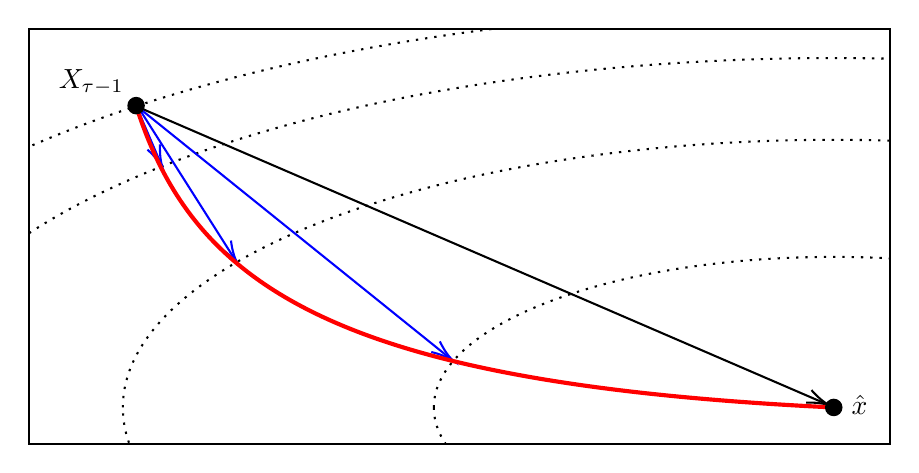
\begin{tikzpicture}[x=0.75pt,y=0.75pt,yscale=-1,xscale=1]
%uncomment if require: \path (0,224); %set diagram left start at 0, and has height of 224

\draw (150,10) rectangle (565,210);
\clip (150,10) rectangle (565,210);

%Shape: Ellipse [id:dp1243945339573651] 
\draw  [dash pattern={on 0.84pt off 2.51pt}] (345.17,192.48) .. controls (345.17,152.42) and (431.44,119.94) .. (537.86,119.94) .. controls (644.27,119.94) and (730.54,152.42) .. (730.54,192.48) .. controls (730.54,232.55) and (644.27,265.02) .. (537.86,265.02) .. controls (431.44,265.02) and (345.17,232.55) .. (345.17,192.48) -- cycle ;
%Shape: Ellipse [id:dp7279543966183535] 
\draw  [dash pattern={on 0.84pt off 2.51pt}] (195.35,192.48) .. controls (195.35,121.27) and (348.7,63.53) .. (537.86,63.53) .. controls (727.01,63.53) and (880.36,121.27) .. (880.36,192.48) .. controls (880.36,263.7) and (727.01,321.43) .. (537.86,321.43) .. controls (348.7,321.43) and (195.35,263.7) .. (195.35,192.48) -- cycle ;
%Shape: Ellipse [id:dp834765959265189] 
\draw  [dash pattern={on 0.84pt off 2.51pt}] (90.68,192.48) .. controls (90.68,99.5) and (290.89,24.13) .. (537.86,24.13) .. controls (784.83,24.13) and (985.04,99.5) .. (985.04,192.48) .. controls (985.04,285.46) and (784.83,360.84) .. (537.86,360.84) .. controls (290.89,360.84) and (90.68,285.46) .. (90.68,192.48) -- cycle ;
%Shape: Ellipse [id:dp7198209862993796] 
\draw  [dash pattern={on 0.84pt off 2.51pt}] (26.37,192.48) .. controls (26.37,86.13) and (255.37,-0.08) .. (537.86,-0.08) .. controls (820.34,-0.08) and (1049.34,86.13) .. (1049.34,192.48) .. controls (1049.34,298.83) and (820.34,385.05) .. (537.86,385.05) .. controls (255.37,385.05) and (26.37,298.83) .. (26.37,192.48) -- cycle ;
%Straight Lines [id:da017585193024664658] 
\draw    (202.73,47.77) -- (534.02,190.69) ;
\draw [shift={(535.86,191.48)}, rotate = 203.34] [color={rgb, 255:red, 0; green, 0; blue, 0 }  ][line width=0.75]    (10.93,-3.29) .. controls (6.95,-1.4) and (3.31,-0.3) .. (0,0) .. controls (3.31,0.3) and (6.95,1.4) .. (10.93,3.29)   ;
%Straight Lines [id:da7563818207961095] 
\draw [color={rgb, 255:red, 0; green, 0; blue, 255 }  ,draw opacity=1 ]   (202.73,47.77) -- (249.45,121.36) ;
\draw [shift={(250.52,123.05)}, rotate = 237.59] [color={rgb, 255:red, 0; green, 0; blue, 255 }  ,draw opacity=1 ][line width=0.75]    (10.93,-3.29) .. controls (6.95,-1.4) and (3.31,-0.3) .. (0,0) .. controls (3.31,0.3) and (6.95,1.4) .. (10.93,3.29)   ;
%Straight Lines [id:da7413802748055005] 
\draw [color={rgb, 255:red, 0; green, 0; blue, 255 }  ,draw opacity=1 ]   (201.73,47.05) -- (213.74,75.21) ;
\draw [shift={(214.52,77.05)}, rotate = 246.91] [color={rgb, 255:red, 0; green, 0; blue, 255 }  ,draw opacity=1 ][line width=0.75]    (10.93,-3.29) .. controls (6.95,-1.4) and (3.31,-0.3) .. (0,0) .. controls (3.31,0.3) and (6.95,1.4) .. (10.93,3.29)   ;
%Straight Lines [id:da4342657875617628] 
\draw [color={rgb, 255:red, 0; green, 0; blue, 255 }  ,draw opacity=1 ]   (201.73,47.05) -- (352.97,168.79) ;
\draw [shift={(354.52,170.05)}, rotate = 218.82999999999998] [color={rgb, 255:red, 0; green, 0; blue, 255 }  ,draw opacity=1 ][line width=0.75]    (10.93,-3.29) .. controls (6.95,-1.4) and (3.31,-0.3) .. (0,0) .. controls (3.31,0.3) and (6.95,1.4) .. (10.93,3.29)   ;
%Curve Lines [id:da6506967535871442] 
\draw [color={rgb, 255:red, 255; green, 0; blue, 0 }  ,draw opacity=1 ][line width=1.5]    (201.73,47.05) .. controls (229.52,135.05) and (299.52,181.05) .. (537.86,192.48) ;
%Shape: Ellipse [id:dp6733708115016783] 
\draw  [fill={rgb, 255:red, 0; green, 0; blue, 0 }  ,fill opacity=1 ] (198.02,47.05) .. controls (198.02,45) and (199.68,43.34) .. (201.73,43.34) .. controls (203.79,43.34) and (205.45,45) .. (205.45,47.05) .. controls (205.45,49.11) and (203.79,50.77) .. (201.73,50.77) .. controls (199.68,50.77) and (198.02,49.11) .. (198.02,47.05) -- cycle ;
%Shape: Ellipse [id:dp7361874596461209] 
\draw  [fill={rgb, 255:red, 0; green, 0; blue, 0 }  ,fill opacity=1 ] (534.14,192.48) .. controls (534.14,190.43) and (535.8,188.76) .. (537.86,188.76) .. controls (539.91,188.76) and (541.57,190.43) .. (541.57,192.48) .. controls (541.57,194.53) and (539.91,196.2) .. (537.86,196.2) .. controls (535.8,196.2) and (534.14,194.53) .. (534.14,192.48) -- cycle ;

% Text Node
\draw (545,185) node [anchor=north west][inner sep=0.75pt]    {$\hat{x}$};
% Text Node
\draw (163,28) node [anchor=north west][inner sep=0.75pt]    {$X_{\tau -1}$};


\end{tikzpicture}

    \caption{Level sets of $f_{\tau}$ in two dimensions. The blue arrows show projections of $X_{\tau-1}$ onto some level set. The red line visualizes the projection of $X_{\tau-1}$ onto all level sets $\{x \in \mathbb{R}^2 \mid f_{\tau}(x) = l\}$ for $l \in [\hat{x}, f_{\tau}(X_{\tau-1})]$. The step in the direction of the minimizer of $f_{\tau}$ is shown in black. Note that it is not optimal to move directly in the direction of the minimizer as there likely exists a closer point on the same level set. Online balanced descent picks a point on the red line.}
    \label{fig:level_sets_of_the_hitting_costs}
\end{figure}

The mirror descent framework is an extension of gradient descent, allowing to adapt to the underlying ``geometry'' of a problem~\cite{Gupta2020}. The original gradient descent algorithm uses Euclidean geometry. This is shown by a slightly modified form of its update rule: \begin{align*}
    X_{\tau} = \argmin_{x \in \mathcal{X}} \eta_{\tau-1} \langle\nabla f_{\tau-1}(X_{\tau-1}), x\rangle + \frac{1}{2} \norm{x - X_{\tau-1}}_2^2.
\end{align*} Observe that OGD uses the squared Euclidean distance as a regularizer (i.e., a function ensuring that we remain close to the point $X_{\tau-1}$) which can be replaced by another distance to obtain different algorithms~\cite{Gupta2020}.

\paragraph{Proximal Point View} The Bregman divergence is a commonly used class of distance functions. Given a strictly convex \emph{distance-generating function}\index{distance-generating function} $h$, the Bregman divergence measures the deviation of $h$ from its linear approximation.

\begin{definition}\index{Bregman divergence}
\cite{Goel2018} The Bregman divergence from a point $x$ to a point $y$ with respect to a strictly convex function $h$ is given as \begin{align*}
    D_h(x,y) = h(x) - h(y) - \langle\nabla h(y), x - y\rangle.
\end{align*}
\end{definition}

\begin{figure}
    \centering
    


\tikzset{every picture/.style={line width=0.75pt}} %set default line width to 0.75pt        

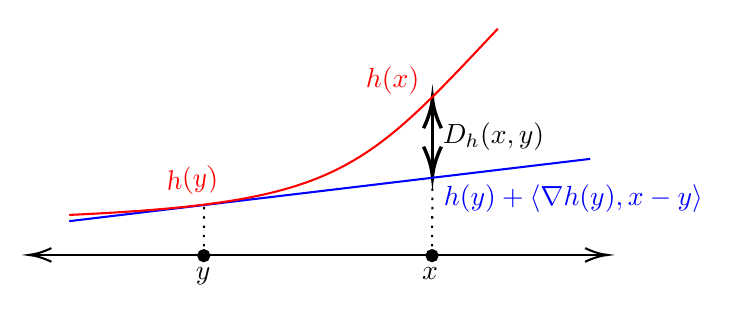
\begin{tikzpicture}[x=0.75pt,y=0.75pt,yscale=-1,xscale=1]
%uncomment if require: \path (0,308); %set diagram left start at 0, and has height of 308

%Straight Lines [id:da8132100594867722] 
\draw    (73,200.33) -- (348,200.33) ;
\draw [shift={(350,200.33)}, rotate = 180] [color={rgb, 255:red, 0; green, 0; blue, 0 }  ][line width=0.75]    (10.93,-3.29) .. controls (6.95,-1.4) and (3.31,-0.3) .. (0,0) .. controls (3.31,0.3) and (6.95,1.4) .. (10.93,3.29)   ;
\draw [shift={(71,200.33)}, rotate = 0] [color={rgb, 255:red, 0; green, 0; blue, 0 }  ][line width=0.75]    (10.93,-3.29) .. controls (6.95,-1.4) and (3.31,-0.3) .. (0,0) .. controls (3.31,0.3) and (6.95,1.4) .. (10.93,3.29)   ;
%Shape: Circle [id:dp9237316574850754] 
\draw  [fill={rgb, 255:red, 0; green, 0; blue, 0 }  ,fill opacity=1 ] (262.67,200.67) .. controls (262.67,199.19) and (263.86,198) .. (265.33,198) .. controls (266.81,198) and (268,199.19) .. (268,200.67) .. controls (268,202.14) and (266.81,203.33) .. (265.33,203.33) .. controls (263.86,203.33) and (262.67,202.14) .. (262.67,200.67) -- cycle ;
%Shape: Circle [id:dp045787056716331875] 
\draw  [fill={rgb, 255:red, 0; green, 0; blue, 0 }  ,fill opacity=1 ] (152.67,200.67) .. controls (152.67,199.19) and (153.86,198) .. (155.33,198) .. controls (156.81,198) and (158,199.19) .. (158,200.67) .. controls (158,202.14) and (156.81,203.33) .. (155.33,203.33) .. controls (153.86,203.33) and (152.67,202.14) .. (152.67,200.67) -- cycle ;
%Straight Lines [id:da4276666085658716] 
\draw  [dash pattern={on 0.84pt off 2.51pt}]  (155.33,200.67) -- (155.52,176.05) ;
%Straight Lines [id:da6234026284865279] 
\draw  [dash pattern={on 0.84pt off 2.51pt}]  (265.33,200.67) -- (265.52,162.38) ;
%Straight Lines [id:da22897635371079694] 
\draw [line width=1.25]    (265.52,159.38) -- (265.52,128.05) ;
\draw [shift={(265.52,125.05)}, rotate = 450] [color={rgb, 255:red, 0; green, 0; blue, 0 }  ][line width=1.25]    (14.21,-4.28) .. controls (9.04,-1.82) and (4.3,-0.39) .. (0,0) .. controls (4.3,0.39) and (9.04,1.82) .. (14.21,4.28)   ;
\draw [shift={(265.52,162.38)}, rotate = 270] [color={rgb, 255:red, 0; green, 0; blue, 0 }  ][line width=1.25]    (14.21,-4.28) .. controls (9.04,-1.82) and (4.3,-0.39) .. (0,0) .. controls (4.3,0.39) and (9.04,1.82) .. (14.21,4.28)   ;
%Straight Lines [id:da4257640445897286] 
\draw [color=blue  ,draw opacity=1 ]   (90.52,184.05) -- (341.52,154.05) ;
%Curve Lines [id:da37061921880533877] 
\draw [color=red  ,draw opacity=1 ][line width=0.75]    (90.52,181.05) .. controls (219.52,175.05) and (231.52,161.05) .. (297,91.33) ;

% Text Node
\draw (150,205) node [anchor=north west][inner sep=0.75pt]    {$y$};
% Text Node
\draw (259,205) node [anchor=north west][inner sep=0.75pt]    {$x$};
% Text Node
\draw (134.94,158) node [anchor=north west][inner sep=0.75pt]  [color=red  ,opacity=1 ,rotate=-353.99]  {$h( y)$};
% Text Node
\draw (232,108) node [anchor=north west][inner sep=0.75pt]  [color=red  ,opacity=1 ]  {$h( x)$};
% Text Node
\draw (269,135) node [anchor=north west][inner sep=0.75pt]    {$D_{h}( x,y)$};
% Text Node
\draw (269.52,165) node [anchor=north west][inner sep=0.75pt]  [color=blue  ,opacity=1 ]  {$h( y) +\langle \nabla h( y) ,x-y\rangle $};


\end{tikzpicture}

    \caption{Bregman Divergence $D_h(x,y)$ for a function $h : \mathbb{R} \to \mathbb{R}$ \cite{Goel2018}. The Bregman divergence measures how much a function differs at $x$ from its linear approximation at $y$.}
    \label{fig:bregman_divergence}
\end{figure}

The definition of the Bregman divergence of a univariate function $h$ is visualized in \cref{fig:bregman_divergence}.

The modified variant of OGD, which uses a Bregman divergence as a regularizer, is known as \emph{online mirror descent}\index{mirror descent} (OMD) or online proximal gradient descent. Note that OMD is parametrized by $h$, which is used to describe the underlying geometry of the problem~\cite{Goel2018}.

For the function $h(x) = \frac{1}{2} \norm{x}_2^2$ from $\mathbb{R}^d$ to $\mathbb{R}$ (the \emph{squared $\ell_2$ norm}\index{squared $\ell_2$ norm}), the Bregman divergence is the Euclidean distance, i.e. $D_h(x,y) = \frac{1}{2} \norm{x-y}_2^2$~\cite{Goel2018}. Hence, OMD reduces to OGD if it is parametrized with the provided definition of $h$, i.e., a Euclidean geometry is used.

\paragraph{Mirror Map View} The proximal point view gives just one perspective of mirror descent. Another perspective that is used frequently is the perspective of mirror maps.

Recall that in OGD, starting from some point $X_{\tau-1}$, we moved into the direction of the gradient of $f$. However, note that $\nabla f_{\tau-1}(X_{\tau-1})$ belongs to the dual space\footnote{The \emph{dual space}\index{dual space} of a vector space $V$ over some field $\mathbb{F}$ is the set of all linear maps from vectors in $V$ to scalars in $\mathbb{F}$ (which are called \emph{linear functionals}\index{linear functionals})~\cite{Wadsley2015}} of $\mathbb{R}^d$. In the Euclidean space, this is not a problem as the dual space of the Euclidean space is the Euclidean space itself~\cite{Gupta2020}. However, when working with normed spaces that are not self-dual, this might be problematic.

Instead of adding elements from the dual space to elements from the primal space, mirror descent maps points from the primal space to the dual space, performs the gradient step in the dual space, and then maps the resulting point back to the primal space.

\begin{figure}
    \centering
    


\tikzset{every picture/.style={line width=0.75pt}} %set default line width to 0.75pt        

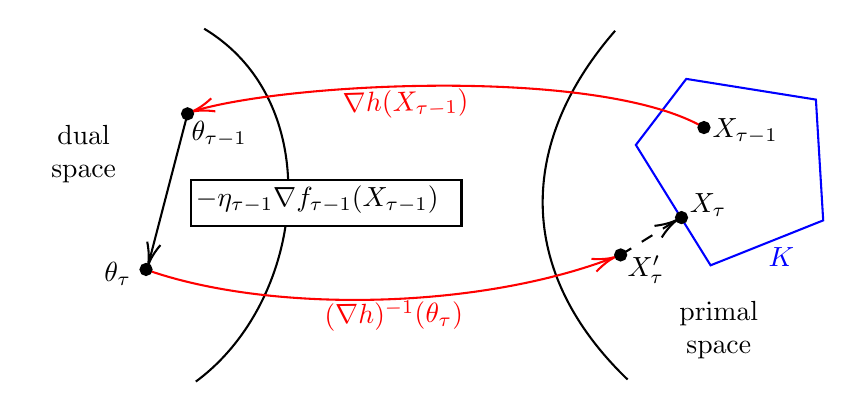
\begin{tikzpicture}[x=0.75pt,y=0.75pt,yscale=-1,xscale=1]
%uncomment if require: \path (0,308); %set diagram left start at 0, and has height of 308

%Curve Lines [id:da740927750098304] 
\draw    (114.52,43.05) .. controls (174.52,79.05) and (163.52,174.05) .. (110.52,213.05) ;
%Curve Lines [id:da195036215046134] 
\draw    (312.52,44.05) .. controls (265.52,98.05) and (264.52,160.05) .. (318.52,212.05) ;
%Shape: Boxed Polygon [id:dp43263390268315804] 
\draw  [color=blue,draw opacity=1 ] (412.78,135.4) -- (358.52,157.05) -- (322.52,99.05) -- (346.81,67.23) -- (409.27,77.2) -- cycle ;
%Curve Lines [id:da4073635308662522] 
\draw [color=red  ,draw opacity=1 ]   (110.58,82.42) .. controls (157.06,68.82) and (305.29,61.49) .. (355.33,90.67) ;
\draw [shift={(108.52,83.05)}, rotate = 342.35] [color=red  ,draw opacity=1 ][line width=0.75]    (10.93,-3.29) .. controls (6.95,-1.4) and (3.31,-0.3) .. (0,0) .. controls (3.31,0.3) and (6.95,1.4) .. (10.93,3.29)   ;
%Shape: Circle [id:dp9467983506453392] 
\draw  [fill={rgb, 255:red, 0; green, 0; blue, 0 }  ,fill opacity=1 ] (103.86,84.05) .. controls (103.86,82.57) and (105.05,81.38) .. (106.52,81.38) .. controls (108,81.38) and (109.19,82.57) .. (109.19,84.05) .. controls (109.19,85.52) and (108,86.71) .. (106.52,86.71) .. controls (105.05,86.71) and (103.86,85.52) .. (103.86,84.05) -- cycle ;
%Shape: Circle [id:dp9056670319943894] 
\draw  [fill={rgb, 255:red, 0; green, 0; blue, 0 }  ,fill opacity=1 ] (352.67,90.67) .. controls (352.67,89.19) and (353.86,88) .. (355.33,88) .. controls (356.81,88) and (358,89.19) .. (358,90.67) .. controls (358,92.14) and (356.81,93.33) .. (355.33,93.33) .. controls (353.86,93.33) and (352.67,92.14) .. (352.67,90.67) -- cycle ;
%Straight Lines [id:da7607534724135314] 
\draw    (106.52,84.05) -- (88.03,155.11) ;
\draw [shift={(87.52,157.05)}, rotate = 284.59000000000003] [color={rgb, 255:red, 0; green, 0; blue, 0 }  ][line width=0.75]    (10.93,-3.29) .. controls (6.95,-1.4) and (3.31,-0.3) .. (0,0) .. controls (3.31,0.3) and (6.95,1.4) .. (10.93,3.29)   ;
%Curve Lines [id:da4928498947155546] 
\draw [color=red  ,draw opacity=1 ]   (89.19,160.05) .. controls (148.23,179.95) and (246.06,178.44) .. (311.54,153.43) ;
\draw [shift={(312.52,153.05)}, rotate = 518.81] [color=red  ,draw opacity=1 ][line width=0.75]    (10.93,-3.29) .. controls (6.95,-1.4) and (3.31,-0.3) .. (0,0) .. controls (3.31,0.3) and (6.95,1.4) .. (10.93,3.29)   ;
%Shape: Circle [id:dp6963694929251834] 
\draw  [fill={rgb, 255:red, 0; green, 0; blue, 0 }  ,fill opacity=1 ] (83.86,159.05) .. controls (83.86,157.57) and (85.05,156.38) .. (86.52,156.38) .. controls (88,156.38) and (89.19,157.57) .. (89.19,159.05) .. controls (89.19,160.52) and (88,161.71) .. (86.52,161.71) .. controls (85.05,161.71) and (83.86,160.52) .. (83.86,159.05) -- cycle ;
%Shape: Circle [id:dp9345908069488471] 
\draw  [fill={rgb, 255:red, 0; green, 0; blue, 0 }  ,fill opacity=1 ] (312.52,152.05) .. controls (312.52,150.57) and (313.72,149.38) .. (315.19,149.38) .. controls (316.66,149.38) and (317.86,150.57) .. (317.86,152.05) .. controls (317.86,153.52) and (316.66,154.71) .. (315.19,154.71) .. controls (313.72,154.71) and (312.52,153.52) .. (312.52,152.05) -- cycle ;
%Shape: Circle [id:dp26656479634987873] 
\draw  [fill={rgb, 255:red, 0; green, 0; blue, 0 }  ,fill opacity=1 ] (341.86,134.05) .. controls (341.86,132.57) and (343.05,131.38) .. (344.52,131.38) .. controls (346,131.38) and (347.19,132.57) .. (347.19,134.05) .. controls (347.19,135.52) and (346,136.71) .. (344.52,136.71) .. controls (343.05,136.71) and (341.86,135.52) .. (341.86,134.05) -- cycle ;
%Straight Lines [id:da12825213670576918] 
\draw  [dash pattern={on 4.5pt off 4.5pt}]  (315.19,152.05) -- (340.83,136.1) ;
\draw [shift={(342.52,135.05)}, rotate = 508.12] [color={rgb, 255:red, 0; green, 0; blue, 0 }  ][line width=0.75]    (10.93,-3.29) .. controls (6.95,-1.4) and (3.31,-0.3) .. (0,0) .. controls (3.31,0.3) and (6.95,1.4) .. (10.93,3.29)   ;

% Text Node
\draw (385,147) node [anchor=north west][inner sep=0.75pt]  [color=blue  ,opacity=1 ]  {$K$};
% Text Node
\draw (179.66,72) node [anchor=north west][inner sep=0.75pt]  [color=red  ,opacity=1 ,rotate=-358.33]  {$\nabla h( X_{\tau -1})$};
% Text Node
\draw (170.87,173) node [anchor=north west][inner sep=0.75pt]  [color=red  ,opacity=1 ,rotate=-359.31]  {$( \nabla h)^{-1}( \theta _{\tau })$};
% Text Node
\draw (358,85) node [anchor=north west][inner sep=0.75pt]    {$X_{\tau -1}$};
% Text Node
\draw (347,121) node [anchor=north west][inner sep=0.75pt]    {$X_{\tau }$};
% Text Node
\draw (317,151) node [anchor=north west][inner sep=0.75pt]    {$X'_{\tau }$};
% Text Node
\draw (65,154) node [anchor=north west][inner sep=0.75pt]    {$\theta _{\tau }$};
% Text Node
\draw (107,86) node [anchor=north west][inner sep=0.75pt]    {$\theta _{\tau -1}$};
% Text Node
\draw  [fill={rgb, 255:red, 255; green, 255; blue, 255 }  ,fill opacity=1 ]  (108,116.05) -- (238.52,116.05) -- (238.52,138) -- (108,138) -- cycle  ;
\draw (109,117.05) node [anchor=north west][inner sep=0.75pt]    {$-\eta _{\tau -1} \nabla f_{\tau -1}( X_{\tau -1})$};
% Text Node
\draw (30,88) node [anchor=north west][inner sep=0.75pt][align=left] {\begin{minipage}[lt]{37.43pt}\setlength\topsep{0pt}
\begin{center}
dual\\space
\end{center}

\end{minipage}};
% Text Node
\draw (336,173) node [anchor=north west][inner sep=0.75pt][align=left] {\begin{minipage}[lt]{37.43pt}\setlength\topsep{0pt}
\begin{center}
primal\\space
\end{center}

\end{minipage}};


\end{tikzpicture}

    \caption{Visualization of a step of Mirror Descent. The previous point $X_{\tau-1}$ is first mapped to the dual space, $\theta_{\tau-1}$. Then, a step is taken into the direction of the gradient, $\theta_{\tau}$, and the resulting point is mapped back to the primal space. Finally, the resulting point $X'_{\tau}$ is projected back onto the feasible region $K$, resulting in the next point $X_{\tau}$ \cite{Gupta2020}.}
    \label{fig:mirror_descent}
\end{figure}

\begin{definition}\index{mirror map}
\cite{Gupta2020} Given a norm $\norm{\cdot}$ and a differentiable and $\alpha$-strongly convex function $h : \mathbb{R}^d \to \mathbb{R}$, the associated mirror map is $\nabla h : \mathbb{R}^d \to \mathbb{R}^d$ and the inverse mirror map is $(\nabla h)^{-1} : \mathbb{R}^d \to \mathbb{R}^d$.
\end{definition}

For $h(x) = \frac{1}{2} \norm{x}_2^2$ the mirror map and its inverse are the identity map~\cite{Gupta2020}. A complete description of the mirror descent framework is given in \cref{alg:md:omd}. Note that the choice of the mirror map is central as it describes the dual space (also called mirror image) where the gradient step is taken. \Cref{fig:mirror_descent} visualizes a step of mirror descent.

\begin{algorithm}
    \caption{Online Mirror Descent~\cite{Gupta2020}}\label{alg:md:omd}
    \SetKwInOut{Input}{Input}
    \Input{$\tau \in \mathbb{N}, K \subset \mathbb{R}^d, \norm{\cdot}, h \in \mathbb{R}^d \to \mathbb{R}$}
    map to the dual space $\theta_{\tau-1} \gets \nabla h (X_{\tau-1})$\;
    take a gradient step in the dual space $\theta_{\tau} \gets \theta_{\tau-1} - \eta_{\tau-1} \nabla f_{\tau-1}(X_{\tau-1})$\;
    map back to the primal space $X'_{\tau} \gets (\nabla h)^{-1}(\theta_{\tau})$\;
    project $X'_{\tau}$ onto a point $X_{\tau} \in K$ using the Bregman projection $X_{\tau} \gets \Pi_K^h(X'_{\tau})$\;
    \Return $X_{\tau}$\;
\end{algorithm}

\begin{definition}\index{Bregman projection}
\cite{Gupta2020} The Bregman projection of a point $x$ onto a convex set $K \subseteq \mathbb{R}^d$ given the distance-generating function $h$ is \begin{align*}
    \Pi_K^h(x) = \argmin_{y \in K} D_h(y,x).
\end{align*}
\end{definition}

Note that when $h$ is the squared $\ell_2$ norm, the Bregman projection is equivalent to the Euclidean projection. Using finite difference methods, the Bregman projection can be computed similarly to the Euclidean projection, $\epsilon$-optimally in $\mathcal{O}(O_{\epsilon}^d)$ time, assuming the runtime of $h$ is constant.

Next, we describe how the ideas from mirror descent are adapted for the smoothed online convex optimization setting, where agents operate with lookahead $1$ and movement costs need to be considered.

\subsubsection{Online Balanced Descent}\label{section:online_algorithms:md:descent_methods:obd}

The online balanced descent (OBD) algorithms were developed by \citeauthor*{Goel2018}~\cite{Goel2018} are a special case of online mirror descent (OMD) with lookahead $1$. In practice, to achieve the one-step lookahead, OBD moves to a point $X_{\tau}$ on a level set of $f_{\tau}(\cdot)$ such that the step is normal to the contour line of $f_{\tau-1}$. In contrast, OMD steps into a direction that is normal to the contour line of $f_{\tau-1}(X_{\tau-1})$. In other words, OMD takes a step with respect to its starting point on some level set, whereas OBD takes a step with respect to its destination on some level set. \Cref{fig:comparison_of_an_update_of_omd_and_obd} shows how these updates compare.

\begin{figure}
    \begin{subfigure}[b]{\textwidth}
    \centering
    


\tikzset{every picture/.style={line width=0.75pt}} %set default line width to 0.75pt        

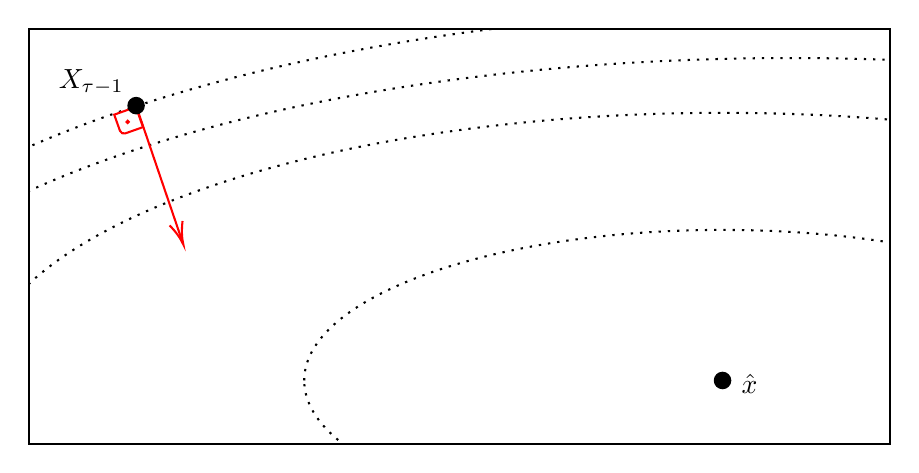
\begin{tikzpicture}[x=0.75pt,y=0.75pt,yscale=-1,xscale=1]
%uncomment if require: \path (0,221); %set diagram left start at 0, and has height of 221

\draw (150,10) rectangle (565,210);
\clip (150,10) rectangle (565,210);

%Shape: Ellipse [id:dp1243945339573651] 
\draw  [dash pattern={on 0.84pt off 2.51pt}] (282.73,179.48) .. controls (282.73,139.42) and (372.97,106.94) .. (484.28,106.94) .. controls (595.59,106.94) and (685.83,139.42) .. (685.83,179.48) .. controls (685.83,219.55) and (595.59,252.02) .. (484.28,252.02) .. controls (372.97,252.02) and (282.73,219.55) .. (282.73,179.48) -- cycle ;
%Shape: Ellipse [id:dp7279543966183535] 
\draw  [dash pattern={on 0.84pt off 2.51pt}] (126.02,179.48) .. controls (126.02,108.27) and (286.42,50.53) .. (484.28,50.53) .. controls (682.14,50.53) and (842.54,108.27) .. (842.54,179.48) .. controls (842.54,250.7) and (682.14,308.43) .. (484.28,308.43) .. controls (286.42,308.43) and (126.02,250.7) .. (126.02,179.48) -- cycle ;
%Shape: Ellipse [id:dp834765959265189] 
\draw  [dash pattern={on 0.84pt off 2.51pt}] (49.52,192.48) .. controls (49.52,99.5) and (258.95,24.13) .. (517.28,24.13) .. controls (775.61,24.13) and (985.04,99.5) .. (985.04,192.48) .. controls (985.04,285.46) and (775.61,360.84) .. (517.28,360.84) .. controls (258.95,360.84) and (49.52,285.46) .. (49.52,192.48) -- cycle ;
%Shape: Ellipse [id:dp7198209862993796] 
\draw  [dash pattern={on 0.84pt off 2.51pt}] (26.37,192.48) .. controls (26.37,86.13) and (255.37,-0.08) .. (537.86,-0.08) .. controls (820.34,-0.08) and (1049.34,86.13) .. (1049.34,192.48) .. controls (1049.34,298.83) and (820.34,385.05) .. (537.86,385.05) .. controls (255.37,385.05) and (26.37,298.83) .. (26.37,192.48) -- cycle ;
%Straight Lines [id:da9739335753395648] 
\draw [color={rgb, 255:red, 255; green, 0; blue, 0 }  ,draw opacity=1 ]   (201.73,47.05) -- (223.88,112.15) ;
\draw [shift={(224.52,114.05)}, rotate = 251.20999999999998] [color={rgb, 255:red, 255; green, 0; blue, 0 }  ,draw opacity=1 ][line width=0.75]    (10.93,-3.29) .. controls (6.95,-1.4) and (3.31,-0.3) .. (0,0) .. controls (3.31,0.3) and (6.95,1.4) .. (10.93,3.29)   ;
%Shape: Ellipse [id:dp7361874596461209] 
\draw  [fill={rgb, 255:red, 0; green, 0; blue, 0 }  ,fill opacity=1 ] (480.56,179.48) .. controls (480.56,177.43) and (482.23,175.76) .. (484.28,175.76) .. controls (486.33,175.76) and (488,177.43) .. (488,179.48) .. controls (488,181.53) and (486.33,183.2) .. (484.28,183.2) .. controls (482.23,183.2) and (480.56,181.53) .. (480.56,179.48) -- cycle ;
%Rounded Single Corner Rect [id:dp48113638837315853] 
\draw  [color={rgb, 255:red, 255; green, 0; blue, 0 }  ,draw opacity=1 ] (196.58,60.42) .. controls (195.51,60.8) and (194.33,60.24) .. (193.95,59.17) -- (191.2,51.41) -- (201.62,47.71) -- (205.06,57.41) -- cycle ;
%Shape: Circle [id:dp7665286358613801] 
\draw  [color={rgb, 255:red, 255; green, 0; blue, 0 }  ,draw opacity=1 ][fill={rgb, 255:red, 0; green, 0; blue, 0 }  ,fill opacity=1 ] (197.15,54.9) .. controls (197.15,54.61) and (197.38,54.38) .. (197.66,54.38) .. controls (197.95,54.38) and (198.18,54.61) .. (198.18,54.9) .. controls (198.18,55.18) and (197.95,55.41) .. (197.66,55.41) .. controls (197.38,55.41) and (197.15,55.18) .. (197.15,54.9) -- cycle ;

%Shape: Ellipse [id:dp6733708115016783] 
\draw  [fill={rgb, 255:red, 0; green, 0; blue, 0 }  ,fill opacity=1 ] (198.02,47.05) .. controls (198.02,45) and (199.68,43.34) .. (201.73,43.34) .. controls (203.79,43.34) and (205.45,45) .. (205.45,47.05) .. controls (205.45,49.11) and (203.79,50.77) .. (201.73,50.77) .. controls (199.68,50.77) and (198.02,49.11) .. (198.02,47.05) -- cycle ;

% Text Node
\draw (492,175) node [anchor=north west][inner sep=0.75pt]    {$\hat{x}$};
% Text Node
\draw (163,28) node [anchor=north west][inner sep=0.75pt]    {$X_{\tau -1}$};

\end{tikzpicture}

    \caption{Update of OMD. The contour lines represent level sets of $f_{\tau-1}$.}
    \end{subfigure}
    \par\bigskip
    \begin{subfigure}[b]{\textwidth}
    \centering
    


\tikzset{every picture/.style={line width=0.75pt}} %set default line width to 0.75pt        

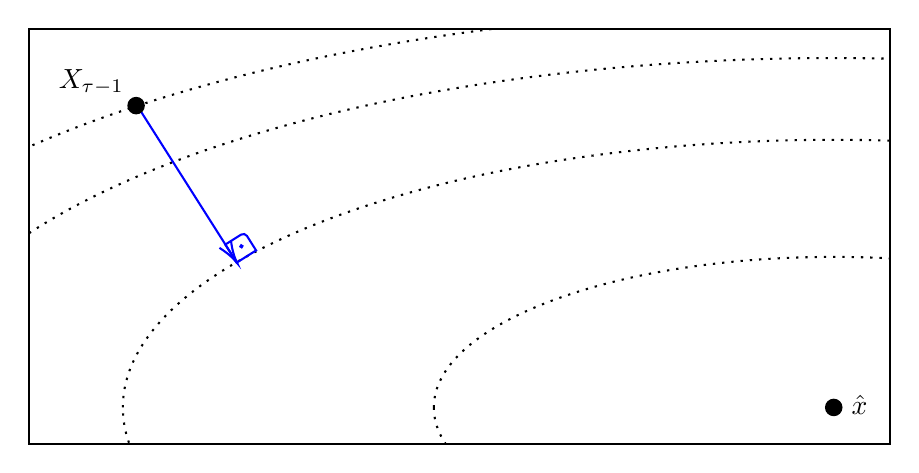
\begin{tikzpicture}[x=0.75pt,y=0.75pt,yscale=-1,xscale=1]
%uncomment if require: \path (0,221); %set diagram left start at 0, and has height of 221

\draw (150,10) rectangle (565,210);
\clip (150,10) rectangle (565,210);

%Shape: Ellipse [id:dp1243945339573651] 
\draw  [dash pattern={on 0.84pt off 2.51pt}] (345.17,192.48) .. controls (345.17,152.42) and (431.44,119.94) .. (537.86,119.94) .. controls (644.27,119.94) and (730.54,152.42) .. (730.54,192.48) .. controls (730.54,232.55) and (644.27,265.02) .. (537.86,265.02) .. controls (431.44,265.02) and (345.17,232.55) .. (345.17,192.48) -- cycle ;
%Shape: Ellipse [id:dp7279543966183535] 
\draw  [dash pattern={on 0.84pt off 2.51pt}] (195.35,192.48) .. controls (195.35,121.27) and (348.7,63.53) .. (537.86,63.53) .. controls (727.01,63.53) and (880.36,121.27) .. (880.36,192.48) .. controls (880.36,263.7) and (727.01,321.43) .. (537.86,321.43) .. controls (348.7,321.43) and (195.35,263.7) .. (195.35,192.48) -- cycle ;
%Shape: Ellipse [id:dp834765959265189] 
\draw  [dash pattern={on 0.84pt off 2.51pt}] (90.68,192.48) .. controls (90.68,99.5) and (290.89,24.13) .. (537.86,24.13) .. controls (784.83,24.13) and (985.04,99.5) .. (985.04,192.48) .. controls (985.04,285.46) and (784.83,360.84) .. (537.86,360.84) .. controls (290.89,360.84) and (90.68,285.46) .. (90.68,192.48) -- cycle ;
%Shape: Ellipse [id:dp7198209862993796] 
\draw  [dash pattern={on 0.84pt off 2.51pt}] (26.37,192.48) .. controls (26.37,86.13) and (255.37,-0.08) .. (537.86,-0.08) .. controls (820.34,-0.08) and (1049.34,86.13) .. (1049.34,192.48) .. controls (1049.34,298.83) and (820.34,385.05) .. (537.86,385.05) .. controls (255.37,385.05) and (26.37,298.83) .. (26.37,192.48) -- cycle ;
%Straight Lines [id:da7563818207961095] 
\draw [color={rgb, 255:red, 0; green, 0; blue, 255 }  ,draw opacity=1 ]   (202.73,47.77) -- (249.45,121.36) ;
\draw [shift={(250.52,123.05)}, rotate = 237.59] [color={rgb, 255:red, 0; green, 0; blue, 255 }  ,draw opacity=1 ][line width=0.75]    (10.93,-3.29) .. controls (6.95,-1.4) and (3.31,-0.3) .. (0,0) .. controls (3.31,0.3) and (6.95,1.4) .. (10.93,3.29)   ;
%Shape: Ellipse [id:dp7361874596461209] 
\draw  [fill={rgb, 255:red, 0; green, 0; blue, 0 }  ,fill opacity=1 ] (534.14,192.48) .. controls (534.14,190.43) and (535.8,188.76) .. (537.86,188.76) .. controls (539.91,188.76) and (541.57,190.43) .. (541.57,192.48) .. controls (541.57,194.53) and (539.91,196.2) .. (537.86,196.2) .. controls (535.8,196.2) and (534.14,194.53) .. (534.14,192.48) -- cycle ;
%Rounded Single Corner Rect [id:dp7003229861226541] 
\draw  [color={rgb, 255:red, 0; green, 0; blue, 255 }  ,draw opacity=1 ] (252.32,109.2) .. controls (253.29,108.6) and (254.56,108.89) .. (255.16,109.85) -- (259.55,116.82) -- (250.19,122.71) -- (244.71,114) -- cycle ;
%Shape: Circle [id:dp9993518534510271] 
\draw  [color={rgb, 255:red, 0; green, 0; blue, 255 }  ,draw opacity=1 ][fill={rgb, 255:red, 0; green, 0; blue, 0 }  ,fill opacity=1 ] (252.97,114.72) .. controls (253.04,114.99) and (252.86,115.27) .. (252.59,115.33) .. controls (252.31,115.39) and (252.04,115.22) .. (251.98,114.94) .. controls (251.91,114.67) and (252.09,114.39) .. (252.36,114.33) .. controls (252.64,114.27) and (252.91,114.44) .. (252.97,114.72) -- cycle ;

%Shape: Ellipse [id:dp6733708115016783] 
\draw  [fill={rgb, 255:red, 0; green, 0; blue, 0 }  ,fill opacity=1 ] (198.02,47.05) .. controls (198.02,45) and (199.68,43.34) .. (201.73,43.34) .. controls (203.79,43.34) and (205.45,45) .. (205.45,47.05) .. controls (205.45,49.11) and (203.79,50.77) .. (201.73,50.77) .. controls (199.68,50.77) and (198.02,49.11) .. (198.02,47.05) -- cycle ;

% Text Node
\draw (545,185) node [anchor=north west][inner sep=0.75pt]    {$\hat{x}$};
% Text Node
\draw (163,28) node [anchor=north west][inner sep=0.75pt]    {$X_{\tau -1}$};

\end{tikzpicture}

    \caption{Update of OBD. The contour lines represent level sets of $f_{\tau}$.}
    \end{subfigure}
    \caption{Comparison of an update of OMD and OBD in two dimensions assuming the distance-generating function $h(x) = \frac{1}{2} \norm{x}_2^2$. OMD (red) takes a step in a direction normal to the contour line of $f_{\tau-1}$ at $X_{\tau-1}$. OBD (blue) takes a step in a direction normal to the contour line of $f_{\tau}$ at $X_{\tau}$ \cite{Goel2018}. The step in the direction of the minimizer of $f_{\tau}$ is shown in black. Note that it is not optimal to move in the direction of the minimizer to a point on some level set as there likely exists a closer point on the same level set.}
    \label{fig:comparison_of_an_update_of_omd_and_obd}
\end{figure}

The algorithmic framework for OBD can roughly be divided into two parts. First, the projection of the previous point onto some level set of the cost function.  Second, the strategies to choose the specific level set and geometry to balance hitting costs and movement costs. The algorithm for (1) is also called the \emph{meta} algorithm as it is parametrized with a concrete level set and geometry (i.e., mirror map).

\subsubsection{Meta Algorithm}

Similar to OMD, the meta algorithm of OBD chooses the next point $X_{\tau}$ in the dual space. However, whereas OMD takes an arbitrary step into the direction of the gradient, OBD takes the shortest step into some sub-level set $K_l = \{x \in \mathcal{X} \mid f_{\tau}(x) \leq l\}$ of the revealed hitting cost $f_{\tau}$. In other words, we seek to find the Bregman projection of $X_{\tau-1}$ onto the sub-level set $K_l$. The first-order condition of the corresponding optimization in the dual space implies that \begin{align}\label{eq:pbd:first_order_condition}
    \nabla h(X_{\tau}) = \nabla h(X_{\tau-1}) - \eta_{\tau} \nabla f_{\tau}(X_{\tau})
\end{align} must be satisfied by $X_{\tau}$ where $\eta_{\tau}$ is the optimal slack of the inequality constraint $f_{\tau}(x) \leq l$~\cite{Goel2018}. Note that this corresponds to a variant of OMD with lookahead $1$.

OBD requires $h$ to be $\alpha$-strongly convex and $\beta$-Lipschitz smooth in the norm $\norm{\cdot}$ that is used to obtain the movement costs. The meta algorithm is described in \cref{alg:md:obd}.

\begin{algorithm}
    \caption{Online Balanced Descent (meta algorithm)~\cite{Goel2018}}\label{alg:md:obd}
    \SetKwInOut{Input}{Input}
    \Input{$\mathcal{I}_{\text{SCO}} = (\tau \in \mathbb{N}, \mathcal{X} \subset \mathbb{R}^d, \norm{\cdot}, (f_1, \dots, f_{\tau}) \in (\mathcal{X} \to \mathbb{R}_{\geq 0})^{\tau}), l \geq 0, \text{distance-generating function } h$}
    $X_{\tau} \gets \Pi_{K_l}^h(X_{\tau-1})$\;
    \Return $X_{\tau}$\;
\end{algorithm}

As an example, we consider the Euclidean space with the $\ell_2$ norm. In this setting $h(x) = \frac{1}{2} \norm{x}_2^2$ is 1-strongly convex and 1-Lipschitz smooth~\cite{Goel2018}. As the corresponding mirror map, $\nabla h$ is the identity map, the first-order condition \cref{eq:pbd:first_order_condition} reduces to \begin{align*}
    X_{\tau} = X_{\tau-1} - \eta_{\tau} \nabla f_{\tau}(X_{\tau})
\end{align*} corresponding to OGD with lookahead $1$.

We can generally choose $h$ to either perform well for the competitive ratio or regret. In their initial paper, \citeauthor*{Goel2018}~\cite{Goel2018} propose two algorithms that balance hitting and movement costs in the primal and dual space and perform well concerning the competitive ratio and regret, respectively.

\subsubsection{Primal Algorithm}

\emph{Primal online balanced descent} (P-OBD) balances hitting and movement costs in the primal space. Let $\hat{x} = \argmin_{x \in \mathcal{X}} f_{\tau}(x)$ and $x(l) = \text{Meta-OBD}(\mathcal{I}, l, h) = \Pi_{K_l}^h(X_{\tau-1})$. Given some $\beta > 0$, the balance parameter $l$ is chosen such that a balance condition $g(l) = \norm{x(l) - X_{\tau-1}} \leq \beta l$ is satisfied. More formally, $l$ is chosen such that either $x(l) = \hat{x}$ and $g(l) < \beta l$ or $g(l) = \beta l$ hold~\cite{Goel2018}.

\citeauthor*{Goel2018}~\cite{Goel2018} show that the balance function $g(l)$ is continuous in $l$. We observe that $l$ is lower bounded by $f_{\tau}(\hat{x})$. As we assume that $\hat{x}$ is unique, $x(l) = \hat{x}$ iff $l = f_{\tau}(\hat{x})$ and the first condition is fulfilled if and only if $g(f_{\tau}(\hat{x})) < \beta f_{\tau}(\hat{x})$. If the first condition is not satisfied, we can efficiently determine an $l$ fulfilling the second condition using a bracketed root finding method on $g(l) - \beta l$ within the interval $[f_{\tau}(\hat{x}), \gamma]$. Here, it suffices to choose $\gamma$ ``large enough'' to ensure that $g(\gamma) \leq \beta \gamma$. Observe that for $\gamma = f_{\tau}(X_{\tau-1})$, this is trivially satisfied, as $x(\gamma) = X_{\tau-1}$ and as such $g(\gamma) = 0$. The algorithm is described in \cref{alg:md:pobd}.

\begin{algorithm}
    \caption{Primal Online Balanced Descent~\cite{Goel2018}}\label{alg:md:pobd}
    \SetKwInOut{Input}{Input}
    \Input{$\mathcal{I}_{\text{SCO}} = (\tau \in \mathbb{N}, \mathcal{X} \subset \mathbb{R}^d, \norm{\cdot}, (f_1, \dots, f_{\tau}) \in (\mathcal{X} \to \mathbb{R}_{\geq 0})^{\tau}), \beta > 0, \text{distance-generating function } h$}
    $\hat{x} = \argmin_{x \in \mathcal{X}} f_{\tau}(x)$\;
    \If{$g(\hat{x}) \leq \beta f_{\tau}(\hat{x})$}{
        \Return $\hat{x}$\;
    }
    $l \gets $ root of $g(l') - \beta l'$ for $l' \in [f_{\tau}(\hat{x}), f_{\tau}(X_{\tau-1})]$\;
    \Return $\text{Meta-OBD}(\mathcal{I}, l, h)$\;
\end{algorithm}

The balancing is chosen such that the movement cost is upper bounded by the constant $\beta$ times the hitting cost~\cite{Goel2018}.

\citeauthor*{Goel2018}~\cite{Goel2018} show that P-OBD attains a competitive ratio of at most $3 + \mathcal{O}(1 / \alpha)$ for some $\beta > 0$, $\alpha$-locally polyhedral cost functions, and the $\ell_2$ norm as movement cost. They also show that local polyhedrality is useful when other norms like the $l_{\infty}$ norm are used. Note that the algorithm is memoryless and, therefore, nearly optimal, as \citeauthor*{Bansal2015}~\cite{Bansal2015} showed in the uni-dimensional setting that no memoryless algorithm can attain a better competitive ratio than $3$ (which also holds for locally polyhedral cost functions)~\cite{Goel2018}. When used with the $\ell_1$ norm, which is relevant in the application of right-sizing data centers, P-OBD attains a competitive ratio of $\mathcal{O}(\sqrt{d})$ if $\alpha$ is fixed~\cite{Goel2018}. The memoryless algorithm (\cref{alg:ud:memoryless}) of \citeauthor*{Bansal2015}~\cite{Bansal2015} can be seen as a special case of P-OBD for $d = 1$ and $\beta = \frac{1}{2}$~\cite{Goel2018}.

The minimizer can be found $\epsilon$-optimally in $\mathcal{O}(C O_{\epsilon}^d)$ time. Assuming the runtime of $h$ is constant, the balance parameter $l$ can be determined $\epsilon$-optimally in $\mathcal{O}(O_{\epsilon}^d R_{\epsilon})$ time. Overall, P-OBD runs in $\mathcal{O}(C O_{\epsilon}^d + O_{\epsilon}^d R_{\epsilon})$ time.

\subsubsection{Dual Algorithm}

\citeauthor*{Goel2018}~\cite{Goel2018} also developed an algorithm called \emph{dual online balanced descent} (D-OBD), which balances the movement cost in the dual space with the gradient of the hitting cost (which is also in the dual space). Before describing the algorithm, we must first describe how the movement cost can be represented in the dual space. We thus introduce the notion of a \emph{dual norm}.

\begin{definition}\index{dual norm}
\cite{Gupta2020} Given some norm $\norm{\cdot}$ on $\mathbb{R}^d$, its dual norm $\norm{\cdot}_*$ is defined as \begin{align*}
    \norm{y}_* = \sup_{x \in \mathbb{R}^d} \{\langle x, y \rangle \mid \norm{x} \leq 1\}.
\end{align*}
\end{definition}

The $\ell_2$ norm is self-dual~\cite{Gupta2020}. In general, the dual norm for a concrete point $y \in \mathbb{R}^d$ can be computed with the following convex optimization: \begin{align*}
    &\max_{x \in \mathbb{R}^d} &&\langle x, y \rangle \\
    &\text{subject to}         &&\norm{x} \leq 1.
\end{align*}

Returning to the description of D-OBD, for some fixed learning rate $\eta$, $l$ is now chosen such that \begin{align*}
    \norm{\nabla h(x(l)) - \nabla h(X_{\tau-1})}_* = \eta \norm{\nabla f_{\tau}(x(l))}_*
\end{align*} holds. Let $g_1(l) = \norm{\nabla h(x(l)) - \nabla h(X_{\tau-1})}_*$ and $g_2(l) = \norm{\nabla f_{\tau}(x(l))}_*$. Again, \citeauthor*{Goel2018}~\cite{Goel2018} show that the balance function $\frac{g_1(l)}{g_2(l)}$ is continuous in $l$ under the assumption that $h$ and $f_{\tau}$ are continuously differentiable on $\mathcal{X}$. Similar to our analysis of P-OBD, we observe  that $l$ is lower bounded by $f_{\tau}(\hat{x})$. We can determine $l$ using a bracketed root finding method on $g_1(l) - \eta g_2(l)$ within the interval $[f_{\tau}(\hat{x}), \gamma]$. We observe that for $l = f_{\tau}(\hat{x})$, $g_1(l) \geq \eta g_2(l) = 0$. Therefore, we need to choose $\gamma$ such that $g_1(l) \leq \eta g_2(l)$ is satisfied. Similar to our argument for P-OBD, it suffices to choose $\gamma = f_{\tau}(X_{\tau-1})$, resulting in $x(\gamma) = X_{\tau-1}$, and implying $g_1(\gamma) = 0$. The resulting algorithm is described in \cref{alg:md:dobd}.

\begin{algorithm}
    \caption{Dual Online Balanced Descent~\cite{Goel2018}}\label{alg:md:dobd}
    \SetKwInOut{Input}{Input}
    \Input{$\mathcal{I}_{\text{SCO}} = (\tau \in \mathbb{N}, \mathcal{X} \subset \mathbb{R}^d, \norm{\cdot}, (f_1, \dots, f_{\tau}) \in (\mathcal{X} \to \mathbb{R}_{\geq 0})^{\tau}), \eta > 0, \text{distance-generating function } h$}
    $\hat{x} = \argmin_{x \in \mathcal{X}} f_{\tau}(x)$\;
    $l \gets $ root of $g_1(l') - \eta g_2(l')$ for $l' \in [f_{\tau}(\hat{x}), f_{\tau}(X_{\tau-1})]$\;
    \Return $\text{Meta-OBD}(\mathcal{I}, l, h)$\;
\end{algorithm}

\citeauthor*{Goel2018}~\cite{Goel2018} show that the $L$-constrained dynamic regret of D-OBD is upper bounded by $\frac{G L}{\eta} + \frac{T \eta}{2 \alpha}$ where $h$ is $\alpha$-strongly convex in $\norm{\cdot}$, $\norm{\nabla h(x)}_*$ is upper bounded by $G$, and $\nabla h(0) = 0$. When $G$, $L$, and $T$ are known, $\eta$ can be chosen optimally as $\eta = \sqrt{\frac{2 G L \alpha}{T}}$, resulting in an $L$-constrained dynamic regret that is upper bounded by $\sqrt{\frac{2 G L T}{\alpha}}$~\cite{Goel2018}. Further, in this setting, D-OBD achieves static regret $\mathcal{O}(\sqrt{T})$~\cite{Goel2018}.

An evaluation of the dual norm can be computed $\epsilon$-optimally in $\mathcal{O_{\epsilon}^d}$ time. Thus, assuming the runtime of $h$ is constant, $l$ can be found in $\mathcal{O}((O_{\epsilon}^d)^2 R_{\epsilon})$ time. Overall, the asymptotic time complexity of D-OBD is given as $\mathcal{O}(C O_{\epsilon}^d + (O_{\epsilon}^d)^2 R_{\epsilon})$.

\subsubsection{Greedy and Regularized Algorithms}

Later, \citeauthor*{Goel2019}~\cite{Goel2019} proposed two additional algorithms using the OBD framework, \emph{greedy online balanced descent} (G-OBD) and \emph{regularized online balanced descent} (R-OBD). Both algorithms yield strong guarantees for the competitive ratio in the setting of squared $\ell_2$ norm movement costs and $\alpha$-strongly convex hitting costs where the optimal competitive ratio is $\mathcal{O}(1 / \sqrt{\alpha})$ as $\alpha$ approaches zero. G-OBD achieves this competitive ratio for quasiconvex\footnote{A function is quasiconvex iff it has a unique global minimum.} hitting costs that are $\alpha$-strongly convex around their minimizer and squared $\ell_2$ norm movement costs. R-OBD achieves this competitive ratio for $\alpha$-strongly convex hitting costs and arbitrary Bregman divergences as movement costs.

Both algorithms take an additional step of size $\mathcal{O}(\sqrt{\alpha})$ towards the minimizer of the hitting cost. G-OBD works by first taking a regular P-OBD step to some level set of the hitting cost. Then, it takes an additional step towards the minimizer of the hitting cost with a step size based on the convexity parameter $\alpha$. In contrast, R-OBD picks the next point by minimizing a weighted sum of hitting and movement costs. It uses an additional regularization term that encourages the algorithm to pick a point closer to the minimizer of the hitting cost~\cite{Goel2019}. We do not discuss G-OBD and R-OBD in more detail, as their theoretical guarantees do not cover the application of right-sizing data centers, but we provide implementations of them.

\section{Predicting}\label{section:online_algorithms:md:predictions}

In practice, we can attempt to use predicted hitting costs to improve the performance of online algorithms. Predicting future incoming loads to a high degree of accuracy in the data-center setting is often possible. Using predicted hitting costs and their uncertainty distributions, online algorithms can make more informed decisions in practice. In this section, we begin by describing approaches for time-series predictions and end with discussing algorithms that use such predictions.

\subsection{Prediction Window}

A natural model to allow incorporating predictions is the use of a finite prediction window $w$. A prediction window bridges the gap between offline and online algorithms. Whereas an online algorithm only knows the hitting costs $f_t$ for $t \in [\tau]$ and an offline algorithm knows the hitting costs $f_t$ for all $t \in [T]$, an online algorithm with \emph{prediction window}\index{prediction window} of length $w$ knows all hitting costs $f_t$ up to $\tau + w$, i.e. $t \in [\tau + w]$. In other words, the prediction window $w$ represents the number of upcoming time slots at which the algorithm is assumed to have perfect knowledge of the future.

\subsubsection{Lazy Capacity Provisioning with Prediction Window}

\citeauthor*{Lin2011}~\cite{Lin2011} extend their algorithm lazy capacity provisioning, which we discussed in \cref{section:online_algorithms:ud:lazy_capacity_provisioning} to support the prediction window by changing the update rule to \begin{align*}
    X_{\tau} = \begin{cases} 
        0 & \tau \leq 0 \\
        (X_{\tau-1})_{X_{\tau+w,\tau}^L}^{X_{\tau+w,\tau}^U} & \tau \geq 1
    \end{cases}
\end{align*}

The optimal schedules now need to obtained for $\tau + w$ rather than $\tau$ time slots. Thus, the time complexity changes to $\mathcal{O}((\tau + w) C O_{\epsilon}^{\tau + w})$ and $\mathcal{O}((\tau + w)^2 C \log_2 m)$ in the fractional and integral case, respectively.

The assumption of perfect knowledge of the future is sure to be violated when an online algorithm is used in practice. Still, \citeauthor*{Lin2011}~\cite{Lin2011} show that lazy capacity provisioning with a prediction window is robust to this assumption in practice. \citeauthor*{Lin2011}~\cite{Lin2011} and \citeauthor*{Albers2018}~\cite{Albers2018} showed that using a finite prediction window does not improve the worst-case performance of the online algorithm for the fractional and integral case, respectively. In other words, the competitive ratio of lazy capacity provisioning is $3$ regardless of whether it uses a finite prediction window. In practice, however, \citeauthor*{Lin2011}~\cite{Lin2011} show that a prediction window significantly improves the algorithm's performance.

There are two main drawbacks to using a finite prediction window. First, predictions windows are finite and typically constrained to a short period as they are assumed to be perfect. In contrast, predictions can be made for much longer time horizons, albeit with decreasing accuracy. Second, it completely disregards any knowledge or assumptions of the certainty and noise of the predictions by assuming the predictions to be perfect.

\subsection{Making Predictions}\label{section:online_algorithms:md:predictions:making_predictions}

There exist multiple paradigms for making time-series predictions. Due to much recent engagement in the field of deep learning generally and time-series predictions specifically, multiple approaches perform well in practical settings. Most algorithms separately tune parameters of individual models for short-term and long-term trends as well as seasonality~\cite{Taylor2017, Hosseini2021}.

A fundamental difference between models is Bayesianness, i.e., whether they use an underlying uncertainty distribution within the model. Facebook's Prophet algorithm is Bayesian, whereas LinkedIn's Greykite algorithm is not~\cite{Taylor2017, Hosseini2021}.

For Bayesian models, online algorithms can use the uncertainty distribution to consider outliers appropriately. For non-Bayesian models, additive white Gaussian noise can be added to the prediction to achieve a similar effect. In general, many strategies can be used to obtain a single representative prediction of the underlying distribution. In our experiments, we use the mean prediction to ensure appropriate consideration of outliers. The median or 90th percentile predictions are alternatives that are more robust to outliers.

Note that, in principle, predictions can be made arbitrarily far into the future. However, at some point, they become too uncertain to be valuable. For example, infeasible load profiles may be assigned a positive probability, which would result an infinite cost if we use the mean to obtain a representative prediction, even if all servers are active. Thus, we also use a prediction window, which needs to be set appropriately to account for the uncertainty distribution of the predicted loads.

\subsection{Receding Horizon Control}

\emph{Receding horizon control}\index{receding horizon control} (RHC) (or \emph{model predictive control}) is a methodology for making decisions based on predictions of the future that is commonly used to control data centers~\cite{Lin2012}. In RHC, an agent predicts their action up to some fixed point in time, referred to as the prediction window. Based on this prediction, the agent adjusts their action for the current time slot. In the next time slot, this process repeats~\cite{Zak2017}.

\citeauthor*{Lin2012}~\cite{Lin2012} previously investigated the performance of RHC in the context of right-sizing data centers. RHC works by solving a convex optimization from time $\tau$ to time $\tau + w$ starting from the initial configuration $X_{\tau-1}$. We set $X_0 = \mathbf{0}$. Similar to our analysis of capacity provisioning in \cref{section:offline_algorithms:ud:capacity_provisioning}, we describe by $X^{\tau}(X_{\tau-1}) \in \mathcal{X}^{w+1}$ the optimal schedule for times $\tau$ through $\tau+w$. This schedule is obtained by minimizing \begin{align}\label{eq:rhc}
    \sum_{t=\tau}^{\tau+w} f_t(X_t) + \norm{X_t - X_{t-1}}
\end{align} over configurations $X_{\tau}, \dots, X_{\tau+w} \in \mathcal{X}$. This optimization has $\mathcal{O}(d w)$ dimensions and thus can be computed $\epsilon$-optimally in $\mathcal{O}(C O_{\epsilon}^{dw})$ time. Now, RHC simply picks the first predicted action. RHC is described in \cref{alg:predictions:rhc}.

\begin{algorithm}
    \caption{Receding Horizon Control~\cite{Lin2012}}\label{alg:predictions:rhc}
    \SetKwInOut{Input}{Input}
    \Input{$\mathcal{I}_{\text{SSCO}} = (\tau \in \mathbb{N}, m \in \mathbb{N}, \beta \in \mathbb{R}_{>0}, (f_1, \dots, f_{\tau}) \in (\mathbb{R}_{\geq 0} \to \mathbb{R}_{\geq 0})^{\tau})$}
    $X_{\tau} = X_{\tau}^{\tau}(X_{\tau-1})$\;
    \Return $X_{\tau}$\;
\end{algorithm}

\citeauthor*{Lin2012}~\cite{Lin2012} prove the competitive ratio of RHC in the application of right-sizing data centers. The show that in the uni-dimensional setting, RHC attains a competitive ratio of $1 + \mathcal{O}(1/w)$ which is strictly better than the optimal competitive ratio (for deterministic algorithms without predictions) of $2$ and $3$ for memoryless algorithms for $w > 1$ and $w > \frac{1}{2}$, respectively. However, in a multi-dimensional setting, RHC is $(1 + \max_{k \in [d]} \beta_k / e_k(0))$-competitive where $\beta_k$ was the switching cost of a server of type $k$ and $e_k(0)$ the average energy cost of an idling server of type $k$. Importantly, this competitive ratio does not depend on the size of the prediction window $w$.

\subsection{Averaging Fixed Horizon Control}

In their paper, \citeauthor*{Lin2012}~\cite{Lin2012} present another algorithm, \emph{averaging fixed horizon control} (AFHC), which attains a competitive ratio of $1 + \max_{k \in [d]} \frac{\beta_k}{(w+1) e_k(0)}$. In particular, AFHC is $(1 + \mathcal{O}(1/w))$-competitive. However, \citeauthor*{Lin2012}~\cite{Lin2012} find that in most realistic settings, RHC performs better than AFHC.

At time $\tau$, AFHC works by performing $w + 1$ individual RHC steps starting from $t_0 = \tau-w$ up to $t_0 = \tau$ and averaging the results. Each individual step is also referred to as an iteration of \emph{fixed horizon control} (FHC).

We describe the sub-iterations of AFHC using $k \in [w+1]$. We set $t_0 = \tau+k-(w+1)$, ensuring that $t_0 \in [\tau-w,\tau]$. We denote by $X^{t_0}(X_{t_0-1}^{(k)})$ the optimal schedule for times $t_0$ through $t_0+w$ which is obtained analogously to \cref{eq:rhc}. We also set $X_t = \mathbf{0}$ and $X_t^{(k)} = \mathbf{0}$ for all $t \leq 0$ and $k \in [w+1]$. AFHC is described in \cref{alg:predictions:afhc}.

\begin{algorithm}
    \caption{Averaging Fixed Horizon Control~\cite{Lin2012}}\label{alg:predictions:afhc}
    \SetKwInOut{Input}{Input}
    \Input{$\mathcal{I}_{\text{SSCO}} = (\tau \in \mathbb{N}, m \in \mathbb{N}, \beta \in \mathbb{R}_{>0}, (f_1, \dots, f_{\tau}) \in (\mathbb{R}_{\geq 0} \to \mathbb{R}_{\geq 0})^{\tau})$}
    \ForEach{$k \in [w+1]$}{
        $t_0 \gets \tau+k-(w+1)$\;
        $X^{(k)} \gets X^{t_0}(X_{t_0-1}^{(k)})$\;
    }
    $X_{\tau} = \frac{1}{w+1} \sum_{k=1}^{w+1} X_{\tau}^{(k)}$\;
    \Return $X_{\tau}$\;
\end{algorithm}

Intuitively, AFHC can be interpreted as performing $w+1$ RHC-steps in parallel, where each RHC starts from a different $t_0 \in [\tau-w,\tau]$, and then averaging all configurations for time $\tau$. Note that RHC is equivalent to the last FHC-step with initial time $t_0 = \tau$, i.e., $k = w+1$. The asymptotic time complexity of AFHC is given as $\mathcal{O}(w C O_{\epsilon}^{dw})$.

\citeauthor*{Chen2015}~\cite{Chen2015} show that AFHC achieves sublinear regret and a constant competitive ratio using a prediction window of constant length. \citeauthor*{Badiei2015}~\cite{Badiei2015} introduce a class of ``forward-looking'' algorithms that can consider cost functions within some prediction window but are only allowed to use a constant limited number of past cost functions. They show that among these algorithms, AFHC achieves optimal regret.

In~\cite{Chen2016}, \citeauthor*{Chen2016} generalize RHC and AFHC to a class of algorithms called \emph{committed horizon control} (CHC), which consist of $v \in [w+1]$ sub-iterations of FHC. Note that RHC corresponds to CHC with parameter $v = 1$, whereas AFHC corresponds to CHC with parameter $v = w+1$. They investigate how $v$ can be chosen optimally based on the noise distribution of predictions.

\citeauthor*{Lin2019}~\cite{Lin2019} extend AFHC to a new algorithm called \emph{synchronized fixed horizon control} (SFHC), which is $(1 + \mathcal{O}(1/w))$-competitive for both convex and non-convex cost functions. \citeauthor*{Li2018}~\cite{Li2018} propose two new gradient-based online algorithms, \emph{receding horizon gradient descent} (RHGD) and \emph{receding horizon accelerated gradient} (RHAG), and show that the dynamic regret of RHAG is near-optimal when compared to a class of online algorithms that includes CHC.

